% Intended LaTeX compiler: xelatex + biber
% Compile with latexmk should Just Work™
% latexmk -xelatex -shell-escape main.tex

\documentclass[12pt, a4paper]{gsdiss}

\author{Samantha Silvestre Nuernberg}
\date{\today}
\title{Farol de Santa Marta Nonprofit Web Application}
\degree{BSc Computer Science}

% You only need this if you are using SVG images, and it relies on the
% available of external programmes like inkscape.
% \usepackage{svg}                % \includesvg

\usepackage{float}              % Custom floats and the H option.
% \usepackage{subfig}             % Combine several figures into one.
% \usepackage{wrapfig}            % For figure placement
% \usepackage{rotating}           % For sideways figures and tables.

% \usepackage{longtable}          % Multipage tables.

\usepackage{amssymb}            % Additional maths symbols.
\usepackage{amsthm}             % For theorems etc.
\usepackage{mathtools}          % amsmath plus fixes.

\usepackage{algorithmic}        % Typeset pseudo-code.
\usepackage[chapter]{algorithm} % Float algorithmic blocks (e.g. add caption).

% Code formatting: Use either listings or minted to typeset code.
\usepackage{listings}
% Minted requires Python and the Pygments package.
% \usepackage{minted}

% More compact lists.
\usepackage{enumitem}
\setlist{nosep}

% Set XeLaTeX or PdfLaTeX options.
\usepackage{iftex}

% XeLaTeX options.
\ifxetex
\usepackage{unicode-math}       % Include unicode characters in
                                % maths.

\usepackage{fontspec}           % For setting fonts.

% Prioritise FOSS fonts.
\IfFontExistsTF{Libertinus Serif}{
  \setmainfont{Libertinus Serif}
}{
  \IfFontExistsTF{Times New Roman}{
    \setmainfont{Times New Roman}
  }{}
}

\IfFontExistsTF{Libertinus Sans}{
  \setsansfont{Libertinus Sans}
}{}

\IfFontExistsTF{Libertinus Math}{
  \setmathfont{Libertinus Math}
}{}

\IfFontExistsTF{Roboto Mono}{
  \setmonofont{Roboto Mono}
}{}

\usepackage{csquotes}           % Context sensitive quotations.
\usepackage{polyglossia}        % Babel replacement for XeLaTex.
\setmainlanguage[variant=uk]{english}
\fi

% PdfLaTeX options.
\ifpdftex
\usepackage[utf8]{inputenc}

% Use Time New Roman clone.
\usepackage{mathptmx}
% Or use newer TX font package.
% \usepackage{newtxtext,newtxmath}

\usepackage[english]{babel}
\fi

% Use biblatex+biber for ACM-like references.
\usepackage[style=numeric,backend=biber]{biblatex}
\DefineBibliographyStrings{english}{%
  bibliography = {References},
}
\ExecuteBibliographyOptions{
  sorting=nyt,
  maxcitenames=2,
  giveninits=true,
  urldate=long,
  doi=true,
  isbn=false,
  eprint=false,
  uniquename=allinit,
  uniquelist=minyear
}

\addbibresource{refs.bib}

\usepackage{hyperref}           % For cross references.
\hypersetup{
 pdfauthor={\theauthor},
 pdftitle={\thetitle},
 pdfkeywords={},
 pdfsubject={},
 pdfcreator={},
 pdflang={British},
 colorlinks,
 linkcolor=blue,
 citecolor=blue,
 urlcolor=gray
}

% Custom latex commands.
% Generic notation
\newcommand{\setof}[1]{\ensuremath{\left \{ #1 \right \}}}
\newcommand{\tuple}[1]{\ensuremath{\left \langle #1 \right \rangle }}
\newcommand{\vecb}[1]{\ensuremath{\mathbf{#1}}}
\newcommand{\matb}[1]{\ensuremath{\mathbf{#1}}}
\DeclareMathOperator*{\argmin}{arg\,min}
\DeclareMathOperator*{\argmax}{arg\,max}

% Pattern discovery
\newcommand{\SIA}{\mbox{\texttt{SIA}}}
\newcommand{\SIATEC}{\mbox{\texttt{SIATEC}}}
\newcommand{\COSIATEC}{\mbox{\texttt{COSIATEC}}}

\newcommand{\patternP}{\ensuremath{P}}
\newcommand{\datasetD}{\ensuremath{D}}
%\newcommand{\Pmtp}{\ensuremath{P_{\textsc{mtp}}}}
\newcommand{\Ptec}{\ensuremath{P'}}
\newcommand{\Ptecn}[1]{\ensuremath{\Ptec_{#1}}}
\newcommand{\tec}{\mathcal{T}}
\newcommand{\translator}{\vecb{t}}
\newcommand{\translatorSetT}{\ensuremath{T}} % set of vectors, not
                                % equiv. to familyF

% Cormen set-cover symbols
\newcommand{\setX}{\ensuremath{X}}
\newcommand{\familyF}{\ensuremath{\mathcal{F}}}
\newcommand{\subsetS}{\ensuremath{S}}
\newcommand{\coverC}{\ensuremath{\mathcal{C}}}
\newcommand{\coverCi}{\ensuremath{\mathcal{C}_{i}}}

% SIA functions
\DeclareMathOperator{\fcoverage}{coverage}
\DeclareMathOperator{\fcoveragei}{coverage_{i}}
%\DeclareMathOperator{\funcovered}{uncovered}
\DeclareMathOperator{\fcompressionratio}{compression\;ratio}
\DeclareMathOperator{\fcompactness}{compactness}
\DeclareMathOperator{\fcompactnesssegv}{compactness-v}
\DeclareMathOperator{\fweight}{weight}

\DeclareMathOperator{\fsegment}{\mathit{segment}}
\DeclareMathOperator{\fsegmentv}{\mathit{segment-v}}
\DeclareMathOperator{\fvoice}{\mathit{voice}}
\DeclareMathOperator{\fvoices}{\mathit{voices}}
\DeclareMathOperator{\fstart}{\mathit{start}}
\DeclareMathOperator{\fend}{\mathit{end}}

\newcommand{\heuristic}{h}
\newcommand{\weightW}{W_{\heuristic}}

% Point set symbolic
\newcommand{\sonset}{\ensuremath{\texttt{onset}}}
\newcommand{\smpitch}{\ensuremath{\texttt{mpitch}}}
\newcommand{\svoice}{\ensuremath{\texttt{voice}}}
\newcommand{\scpitch}{\ensuremath{\texttt{cpitch}}}
\newcommand{\sdur}{\ensuremath{\texttt{dur}}}
\newcommand{\scpint}{\ensuremath{\texttt{cpint}}}
\newcommand{\sioi}{\ensuremath{\texttt{ioi}}}

% Function from sym to geo
% \newcommand{\fioi}{\textit{ioi}}
% \newcommand{\fcpint}{\textit{cpint}}


% Point set geometry
\newcommand{\onset}{\ensuremath{\textsc{onset}}}
\newcommand{\cpitch}{\ensuremath{\textsc{cpitch}}}
\newcommand{\dur}{\ensuremath{\textsc{dur}}}
\newcommand{\cpint}{\ensuremath{\textsc{cpint}}}
\newcommand{\ioi}{\ensuremath{\textsc{ioi}}}

\DeclareMathOperator{\fcpitch}{\mathit{cpitch}}
\DeclareMathOperator{\fdur}{\mathit{dur}}

% Symbolic representation of metre
\newcommand{\TMI}{\ensuremath{\mathcal{T}}}
\DeclareMathOperator{\flabel}{\mathit{label}}
\DeclareMathOperator{\froot}{\mathit{root}}
\DeclareMathOperator{\fdepth}{\mathit{depth}}
\DeclareMathOperator{\flevel}{\mathit{level}}
\DeclareMathOperator{\fparent}{\mathit{parent}}
\DeclareMathOperator{\fchildren}{\mathit{children}}
\DeclareMathOperator{\fisleaf}{\mathit{is-leaf}}
\DeclareMathOperator{\fleafnodes}{\mathit{leaf-nodes}}
\DeclareMathOperator{\fchild}{\mathit{child}}
\DeclareMathOperator{\fheight}{\mathit{height}}
\DeclareMathOperator{\farity}{\mathit{arity}}
\DeclareMathOperator{\fposition}{\mathit{position}}

\DeclareMathOperator{\fpioi}{\mathit{p-ioi}}
\DeclareMathOperator{\fonset}{\mathit{onset}}
\DeclareMathOperator{\faenergy}{\mathit{a-energy}}
\DeclareMathOperator{\fcard}{\mathit{cardinality}}
\DeclareMathOperator{\fmeanpioi}{\mathit{mean-p-ioi}}
\DeclareMathOperator{\fmeanaenergy}{\mathit{mean-a-energy}}

% Conceptual spaces
\newcommand{\metrep}{\textsc{\mbox{metre-p}}}
\newcommand{\metres}{\textsc{\mbox{metre-s}}}
\newcommand{\tempo}{\textsc{\mbox{tempo}}}
\newcommand{\meanPulseIOI}[1]{\ensuremath{\textsc{mean\_p\_ioi}^{#1}}}
\newcommand{\meanAttEnergy}[1]{\ensuremath{\textsc{mean\_a\_energy}^{#1}}}
\newcommand{\cratio}[1]{\ensuremath{\textsc{c\_ratio}^{#1}}}

\newcommand{\pulseIOI}[1]{\ensuremath{\textsc{p\_ioi}^{#1}}}
\newcommand{\attEnergy}[1]{\ensuremath{\textsc{a\_energy}^{#1}}}

\newcommand{\nnk}[1]{\ensuremath{k\text{#1}}}
\newcommand{\mathkequals}[1]{\ensuremath{k\text{~=~#1}}}
\newcommand{\mathnequals}[1]{\ensuremath{n\text{~=~#1}}}

% Algorithms
\DeclareMathOperator{\mapTreeMeanPulseIOI}{\mathtt{MAP\_T\_MEAN\_PIOI}}
\DeclareMathOperator{\mapTreeMeanEnergy}{\mathtt{MAP\_T\_MEAN\_AENERGY}}
\DeclareMathOperator{\mapTreeCRatio}{\mathtt{MAP\_T\_MEAN\_CRATIO}}

\DeclareMathOperator{\mapTreePulseIOI}{\mathtt{MAP\_T\_PIOI}}
%\DeclareMathOperator{\fabsDepthOffset}{\mathtt{ABS\_CYCLE\_DEPTH\_OFFSET}}
\DeclareMathOperator{\fabsDepthOffset}{\mathit{abs-depth-offset}}
%\DeclareMathOperator{\fwithinCycleOffset}{\mathtt{WITHIN\_CYCLE\_NODE\_OFFSET}}
\DeclareMathOperator{\fwithinCycleOffset}{\mathit{within-cycle-offset}}
\DeclareMathOperator{\fillIOIDomain}{\mathtt{FILL\_PIOI\_DOMAIN}}
\DeclareMathOperator{\repeatSubSeq}{\mathtt{REPEAT\_SUB\_SEQ}}
\DeclareMathOperator{\mapTreeAttEnergy}{\mathtt{MAP\_T\_AENERGY}}
\DeclareMathOperator{\fabsWithinNCycleOffset}{\mathit{abs-within-n-cycle-offset}}


% Custom title page.
\renewcommand\maketitle{
  \begin{titlepage}
    \clearpage
    \setlength{\headheight}{37pt}
    \fancyhf{}
    \rhead{
      
\includegraphics[width=50mm]{images/goldsmiths-logo-pantone-442.pdf}
    }
    \renewcommand{\headrulewidth}{0pt}

    \thispagestyle{fancyplain}
    \begin{center}
      \vspace*{1.5in}
      \noindent\begin{minipage}[t]{.85\textwidth}
        \centering\large

        {\LARGE \thetitle}
      \end{minipage}

      \par
      \vspace{1.0in}
      {\large \theauthor}

      \vfill

      \ifdef{\thesupervisor}{\large Supervisor: \thesupervisor}

      \par
      \vspace{1.0in}
      Submitted in partial fulfilment of the requirements\\
      for the degree of \thedegree\\
      of the
      University of London.
      \par
      \vspace{0.25in}
      Department of Computing
      \par
      Goldsmiths, University of London
      \par
      \vspace{0.5in}
      \thedate
    \end{center}
  \end{titlepage}

  \clearpage
  \vspace*{\stretch{2}}
  \begin{center}
    \begin{minipage}{0.7\textwidth}
      \noindent I certify that this dissertation, and the research to which
      it refers, are the result of my own work.
    \end{minipage}
  \end{center}
  \vspace{\stretch{3}}
  \clearpage
}


\begin{document}

\maketitle

\chapter*{Abstract}

The \textit{Praia Limpa Santa Marta} project is a non-profit initiative aimed at addressing the growing environmental challenges faced by the coastal region of Farol de Santa Marta, a popular tourist destination in Southern Brazil. With the influx of visitors, the area has experienced significant environmental degradation, particularly in the form of waste and pollution left on its pristine beaches. This project seeks to develop a comprehensive web platform designed to promote the 'leave no trace' principle, engage the local community, and facilitate sustainable environmental practices. 

The proposed website will serve as a central hub for environmental education, community organization, and fundraising efforts. It will provide resources to educate both locals and tourists about the importance of preserving the natural beauty of the region. Additionally, the platform will enable users to participate in beach clean-up events, contribute to conservation projects through donations, and track the impact of their efforts. 

By leveraging digital tools, \textit{Praia Limpa Santa Marta} aims to transform individual environmental concern into collective action, fostering a culture of sustainability that benefits both the environment and the local economy. The project addresses the critical gap in technical expertise and organizational capacity among local stakeholders, providing them with the necessary resources to effectively manage and sustain conservation efforts. Ultimately, this initiative seeks to ensure the long-term preservation of Farol de Santa Marta's natural landscapes, making it a model for other communities facing similar challenges. 
 
Total Words: 9497


\include{text/0-front-matter/02-acknowledgements}
% \chapter*{Licence}

This work is copyright \copyright \ 2024 Samantha S. Nuernberg, and is licensed
under the Creative Commons Attribution-Share Alike 3.0 Unported
Licence. To view a copy of this licence, visit \\
\url{http://creativecommons.org/licenses/by-sa/3.0/} \\
or send a letter to Creative Commons, 171 Second Street, Suite 300,
San Francisco, California, 94105, USA.

\begin{center}

%	\includegraphics [width =1cm]  {images/cc}
%	\includegraphics [width =1cm]  {images/by}
%	\includegraphics [width =1cm]  {images/sa}

\end{center}

% \chapter*{Related Publications}


\fullcite{foo2017} \\[1ex]


\tableofcontents
%\listoftables
\listoffigures
%\chapter*{List of abbreviations}

\begin{table}[htbp]
  \begin{center}
    \begin{tabular}{ll}

      XXX &	something \\

    \end{tabular}
  \end{center}
\end{table}


% Chapters

\chapter{Introduction}
\label{ch:intro}

 The \textit{Praia Limpa Santa Marta} project represents an innovative response to a pressing environmental issue in the Farol de Santa Marta region, a renowned beach destination in Southern Brazil. Known for its stunning natural landscapes and thriving tourism industry, Farol de Santa Marta faces significant challenges due to the environmental impact of increasing tourist activity. This proposal outlines the development of a non-profit website dedicated to promoting the 'leave no trace' principle and facilitating sustainable practices within the community.

% Choose your own headings.

\section{Motivation}

The motivation for developing the \textit{Praia Limpa Santa Marta} project arises from a significant and urgent need within the community of Farol de Santa Marta. As a region celebrated for its stunning beaches and robust tourist activities, it faces environmental challenges due to the increased influx of tourists. These visitors, while beneficial economically, often leave behind waste, threatening the natural beauty and health of the local ecosystem.
    
    The cleanliness and beauty of Farol de Santa Marta's beaches are not only vital for the local ecosystem but also for the continued attraction of tourists. Tourism is a major economic driver for the community, providing livelihoods and supporting local businesses. Maintaining pristine beaches is crucial for sustaining this economic benefit, as littered and polluted areas could deter visitors and harm the local economy.
    
    A cleaner, well-maintained environment attracts more tourists, which in turn boosts the local economy. Increased tourism leads to more business for local shops, restaurants, and accommodation providers. Additionally, involving the community in conservation efforts can strengthen social bonds and promote a sense of unity and collective purpose. This collaborative spirit can have far-reaching positive effects, enhancing the overall quality of life in Farol de Santa Marta.
    
    Local stakeholders, including small business owners, environmental activists, and residents, have expressed a keen interest in addressing this issue. However, they lack the technical expertise and resources to establish an online platform that could effectively mobilize the community and manage conservation efforts. This gap presents a unique opportunity to leverage web development skills for social and environmental impact.


\section{Aim}

    The project aims to harness this local enthusiasm by providing a tailored web solution that not only raises awareness about the 'leave no trace' principle but also actively engages both locals and tourists in sustainability practices. By creating a platform where community members can learn about environmental preservation, sign up for beach clean-ups, and contribute financially through donations, \textit{Praia Limpa Santa Marta} will empower the community to take ownership of their environment and foster a culture of sustainability.

    This initiative is not just about cleaning up the beaches; it's about building a community-driven movement that ensures the long-term preservation of Farol de Santa Marta's natural landscapes, benefiting both the environment and the local economy reliant on tourism. Through this project, we aim to transform environmental concern into actionable change, making it a compelling venture for anyone passionate about conserving our natural world.

\section{Template Used}


    This project follows the guidelines of the CM3035 Advanced Web Development template titled "Project Idea Title 1: A non-profit web application". The project is structured as a non-profit web application, reflecting a strategic approach to combining web development skills with environmental conservation efforts. The chosen template supports the project's goals by providing a framework that facilitates the development of a user-centric, responsive, and scalable platform that can be easily maintained and adapted for future use.

\chapter{Background}
\label{ch:background}

% Choose your own headings.

\section{Background}

In my researches the non-profit websites that excel tend to have a few key characteristics: clear mission statements, easy navigation, compelling content, and strong calls to action that encourage visitor engagement, such as donations or volunteering.

This review examines related projects, techniques, and methods relevant to this initiative, highlighting the effectiveness and gaps that our project intends to fill.

The \textit{Praia Limpa Santa Marta} project aims to create a non-profit website dedicated to conserving nature and promoting the 'leave no trace' principle in Farol de Santa Marta, Brazil. This review examines related projects, techniques, and methods relevant to this initiative, highlighting the effectiveness and gaps that our project intends to fill.

\section{Literature Review}

The literature review section examines existing research and projects that relate to the objectives of the \textit{Praia Limpa Santa Marta} project, highlighting both their successes and shortcomings to establish a foundation for the proposed initiative.

\subsection{Environmental Conservation and Non-Profit Web Platforms}
Non-profit organizations have increasingly turned to digital platforms to engage the public in environmental conservation efforts. Websites like Charity: Water\cite{charitywater} and World Wildlife Fund\cite{wwf} have set benchmarks in using compelling narratives and visual storytelling to mobilize support and generate donations. Charity: Water, for example, excels in using high-quality imagery and engaging content to communicate its mission of providing clean water in developing countries, as shown in Figure \ref{fig:charity_water}. Similarly, the WWF’s use of powerful imagery and concise messaging effectively advocates for nature conservation, as seen in Figure \ref{fig:WWF}. These examples underscore the importance of clear mission statements, easy navigation, and strong calls to action in non-profit websites.

However, while these platforms have been successful in raising awareness and funds on a global scale, they often lack localized approaches that cater to the specific needs of small communities. For instance, the global reach of the WWF, while impactful, does not necessarily translate into targeted, community-specific actions that are crucial for the success of localized initiatives like \textit{Praia Limpa Santa Marta.} This highlights the need for a platform that combines the strengths of these successful models with a focus on local community engagement and tailored environmental strategies.

\begin{figure}[h]
    \centering
    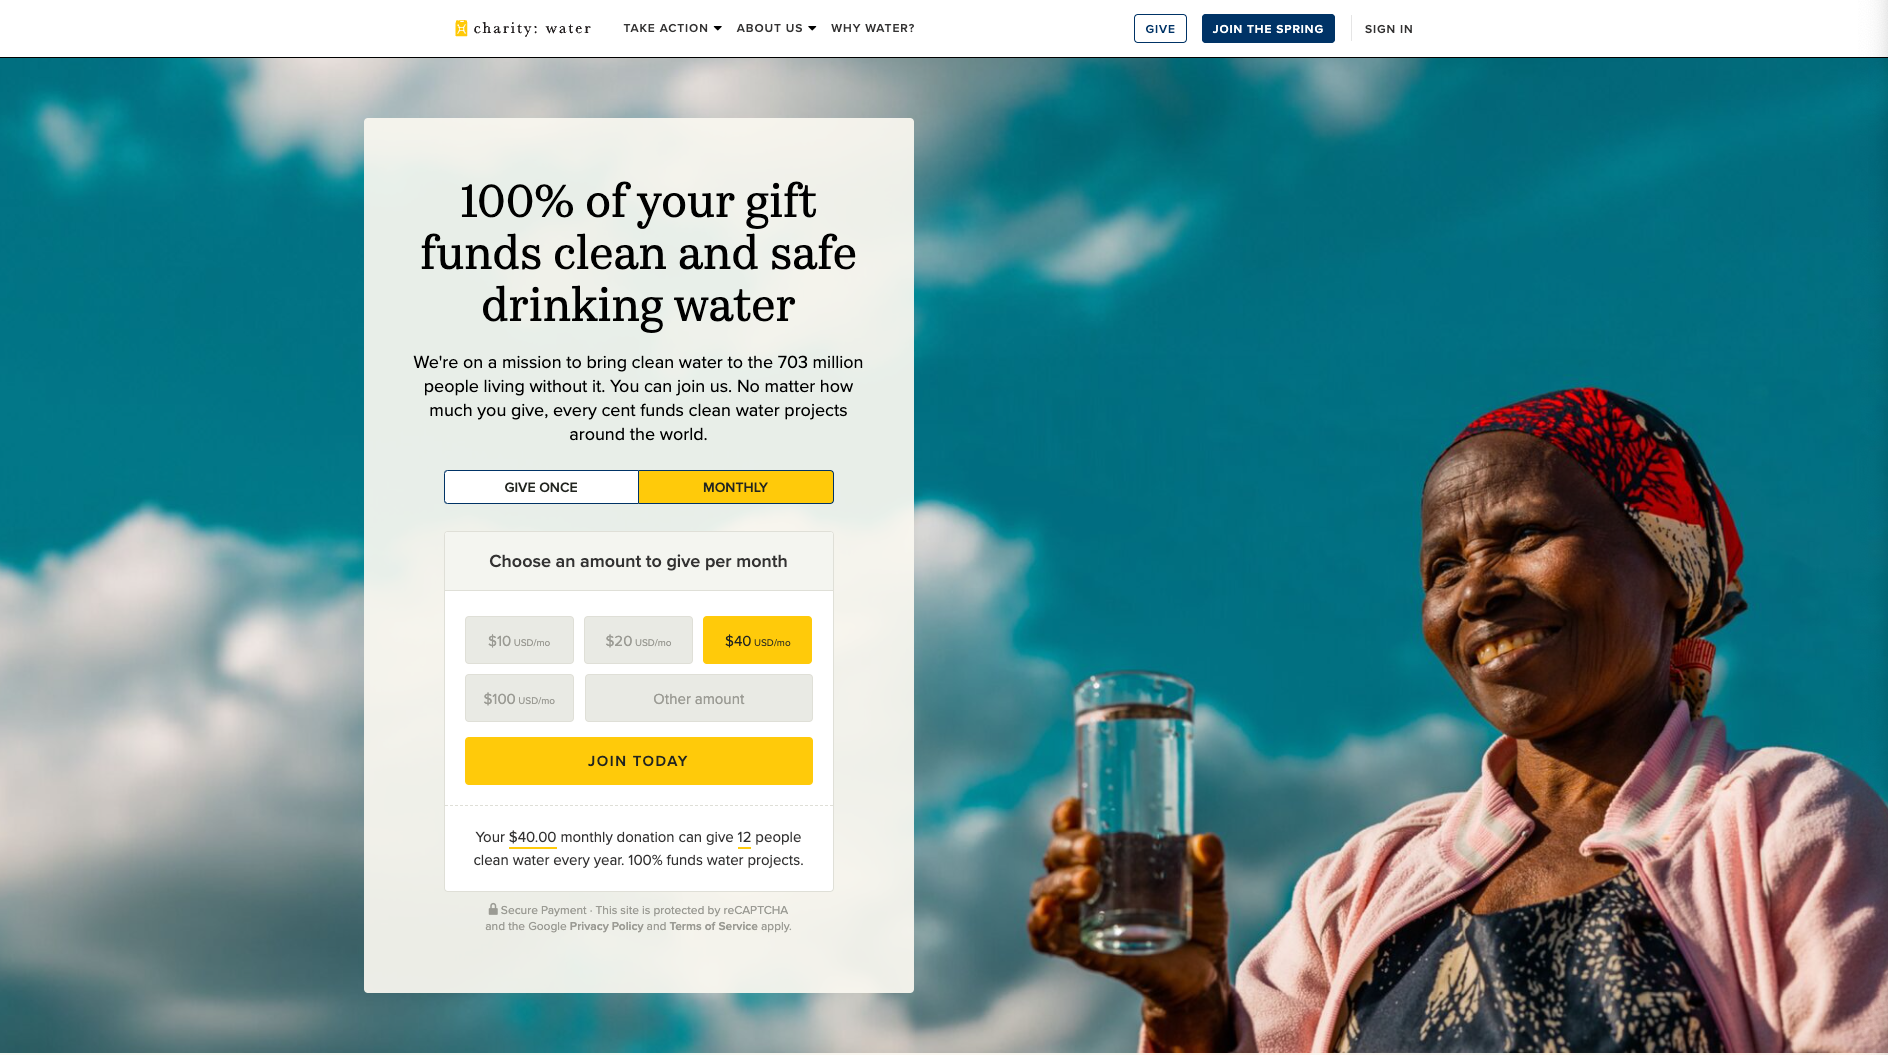
\includegraphics[width=1\linewidth]{images/charity_water.png}
    \caption{Charity: Water}
    \label{fig:charity_water}
\end{figure}

\begin{figure}[h]
    \centering
    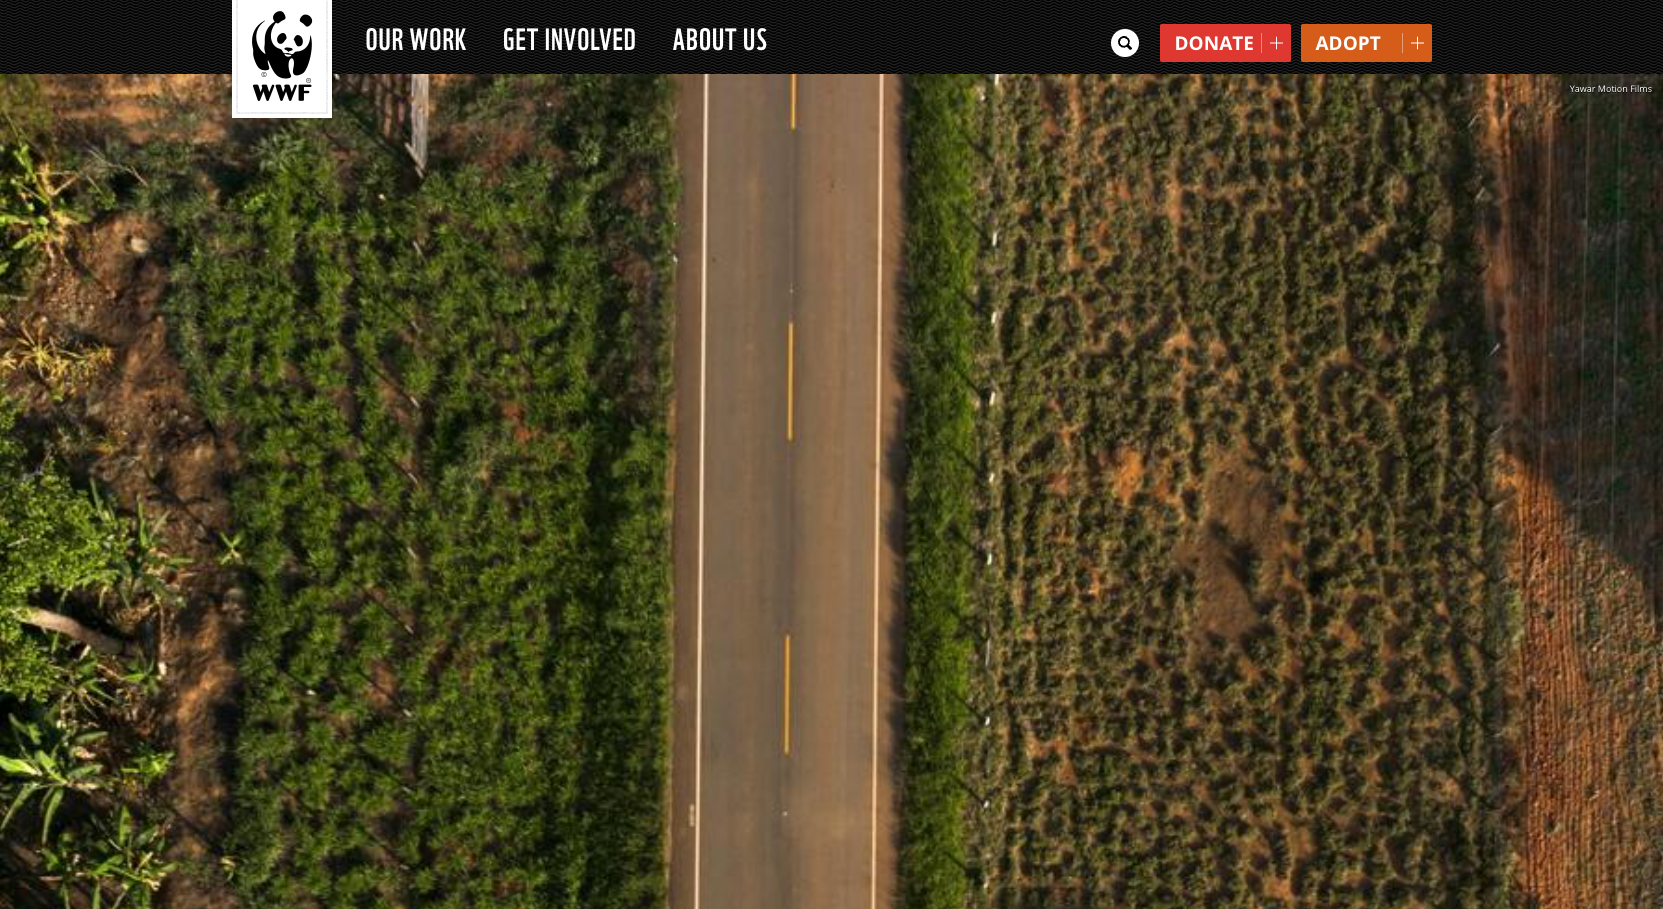
\includegraphics[width=1\linewidth]{images/WWF.png}
    \caption{World Wildlife Fund (WWF)}
    \label{fig:WWF}
\end{figure}



\subsection{Community-Based Conservation Efforts}

The importance of community engagement in conservation efforts cannot be overstated. Studies like those by Western and Wright\cite{western1994} in \textit{Natural Connections: Perspectives in Community-Based Conservation} emphasize the critical role that local communities play in the success of conservation initiatives. The authors argue that sustainable conservation is only possible when the community is actively involved in decision-making and implementation processes. This principle is central to the \textit{Praia Limpa Santa Marta} project, which aims to empower the local community by providing them with the tools and resources necessary to take ownership of their environmental challenges.

Despite the proven importance of community involvement, many conservation projects fail to engage local populations effectively. Initiatives such as the \textit{Beach Clean Brasil} campaign, while successful in mobilizing volunteers, often lack the educational components necessary for fostering long-term environmental stewardship. This gap points to the need for integrating educational programs into the \textit{Praia Limpa Santa Marta} platform to ensure that community members not only participate in clean-up activities but also develop a deeper understanding of the importance of conservation.

\subsection{Tourism and Environmental Impact in Farol de Santa Marta}

Tourism has a profound impact on the social and environmental dynamics of coastal communities like Farol de Santa Marta. The ethnographic research conducted by Santos and Arantes\cite{dosSantos2010} provides valuable insights into how tourism has transformed this traditional fishing village into a popular tourist destination. The influx of tourists has brought economic benefits but also significant environmental challenges, including increased waste and pollution.

The study highlights the need for sustainable tourism practices that balance economic benefits with environmental preservation. This is where the \textit{Praia Limpa Santa Marta} project can make a significant contribution by promoting responsible tourism through its digital platform. By educating tourists about the 'leave no trace' principle and providing them with opportunities to participate in local conservation efforts, the project aims to mitigate the negative environmental impact of tourism in the region.

\subsection{Technological Solutions for Environmental Conservation}

The use of technology in environmental conservation has opened new avenues for engagement and impact. Web-based platforms offer a scalable solution for mobilizing communities, educating the public, and facilitating conservation activities. The choice of Django for the development of the \textit{Praia Limpa Santa Marta} platform reflects a strategic decision to leverage robust and flexible technologies that can handle the complexities of user management, content delivery, and real-time updates.

Previous projects that have successfully integrated technology into conservation efforts, such as the Oceana\cite{oceana} web platform, provide a useful framework for understanding how to maximize the impact of digital tools. However, while Oceana focuses on global ocean conservation, it lacks the localized focus necessary for addressing the specific needs of small communities like Farol de Santa Marta. The \textit{Praia Limpa Santa Marta} project aims to fill this gap by using technology to connect local stakeholders, provide real-time updates on conservation activities, and facilitate easy participation through user-friendly interfaces.

\subsection{Gaps in Current Approaches}

While the reviewed literature and existing projects offer valuable insights, they also reveal significant gaps that \textit{Praia Limpa Santa Marta} aims to address. One of the most prominent gaps is the lack of a strong educational component in many conservation initiatives. While campaigns like Beach Clean Brasil\cite{beachcleanbrasil} are effective in mobilizing volunteers, they do not provide sufficient educational resources to ensure ongoing conservation efforts. The \textit{Praia Limpa Santa Marta} project will incorporate interactive educational content to address this gap, ensuring that both locals and tourists understand the importance of their actions.

Another gap is the limited focus on community engagement in many global conservation projects. While organizations like WWF and Oceana have had global success, their approaches do not always translate to the local level, where community-specific strategies are needed. The \textit{Praia Limpa Santa Marta} platform will prioritize local engagement by involving community members in the planning and implementation of conservation activities, thereby fostering a sense of ownership and responsibility towards the environment.

\subsection{Web Design Insights}

The analysis of various websites reveals the significant role of impactful images as background visuals. Notably, during the Obama election campaign, a comprehensive A/B testing study determined that images were more effective than videos or other types of visuals in generating donations. This research indicated that a clear, compelling image significantly boosts user engagement and donation rates(\cite{kessler2012}). In light of this finding, \textit{Praia Limpa Santa Marta} will feature a clear, vibrant picture of a beach where people are actively engaged in conservation efforts as the primary visual. This approach aims to evoke an emotional connection and prompt visitors to support the cause.

In the 2008 Obama campaign, a significant innovation was the introduction of sequential donation form workflows. Traditionally, clicking a donation button would lead users to a long, intimidating web form. This was especially cumbersome on mobile devices. The new approach broke the form into smaller, manageable sections, guiding users through each step with a "next" button. This method, now common in e-commerce for handling buyer, shipping, and payment information on separate pages, proved that simplifying the donation process into sequential steps increased completion rates and donations.

A key design element identified in successful non-profit websites is the use of pop-ups with pre-selected donation options. This tactic simplifies the donation process and encourages users to contribute by reducing the effort required to make a decision. \textit{Praia Limpa Santa Marta} will implement similar donation pop-ups, ensuring a smooth and user-friendly experience that makes it easy for visitors to support the initiative.

Successful websites often employ a clean, minimalistic design with a central focus on their call to action. By minimizing distractions and using a limited color palette, these websites ensure that users are guided directly towards making a donation. \textit{Praia Limpa Santa Marta} will adopt this design principle, maintaining a clear and straightforward layout that emphasizes the importance of contributing to the conservation efforts.

%%% Local Variables:
%%% mode: latex
%%% TeX-master: "../../main"
%%% End:

\chapter{Specification and design}
\label{ch:specification}

% Choose your own headings.
The design of \textit{Praia Limpa Santa Marta} is focused on creating a platform that meets the specific needs of the Farol de Santa Marta community and its visitors. The following key elements were considered in the design process:


The platform is designed with a user-centric approach, ensuring that it is intuitive and accessible to a diverse audience, including locals, tourists, and environmental activists. Given the varied technical skills of the users, the interface is kept simple yet effective, allowing users of all backgrounds to easily navigate the site and engage with its content.

Considering the international influx of tourists, the platform will support multiple languages, specifically Portuguese and English. This feature is critical for broader accessibility, ensuring that all users, regardless of their native language, can fully engage with the platform. Multilingual support directly addresses the communication needs within the community, facilitating better understanding and participation in conservation activities.

To effectively engage users, the platform includes interactive educational elements such as videos on environmental impact and virtual tours of the beach, which illustrate the effects of littering. These features are designed not only to inform but also to inspire action by demonstrating the importance of conservation efforts in a compelling and immersive way.

Real-time updates are crucial for maintaining community engagement. The platform will provide notifications about upcoming clean-up events and news related to environmental conservation, keeping the community informed and actively involved. This feature supports ongoing participation and fosters a proactive community atmosphere, essential for the success of the conservation initiatives.

\section{System Design}

The system design of the \textit{Praia Limpa Santa Marta} platform is structured to ensure scalability, security, and usability, while meeting the needs of both the local community and visiting tourists. This section outlines the architecture, components, and design considerations that guide the development and deployment of the platform.

\subsection{System Architecture}

The system architecture of \textit{Praia Limpa Santa Marta} is designed to ensure scalability, security, and efficient performance while addressing the needs of the local community and international visitors. The architecture follows a three-tier model, which divides the system into three distinct layers: the presentation layer (frontend), the application layer (backend), and the data layer (database). This separation of concerns facilitates easier maintenance, enhances security, and supports scalability as the project evolves.

\subsection{Presentation Layer (Frontend)}

The presentation layer is responsible for the user interface (UI) and user experience (UX). It is the layer that interacts directly with the users, ensuring that the platform is intuitive, responsive, and accessible across different devices. The key technologies used in this layer include HTML5, CSS3, JavaScript, and Bootstrap.

\begin{itemize}
    \item \textbf{HTML5:} HTML5\cite{html5} is the latest version of the Hypertext Markup Language used to structure content on the web. It provides the semantic foundation for the web pages, ensuring that the content is organized logically and can be easily interpreted by both browsers and search engines. HTML5 supports multimedia elements such as video and audio, and its enhanced features enable the creation of complex web pages without relying heavily on external plugins.

    \item \textbf{CSS3:} CSS3\cite{css3} (Cascading Style Sheets) is used to control the presentation and layout of the web pages. It ensures that the site is visually appealing and responsive, adapting seamlessly to different screen sizes and devices, including desktops, tablets, and smartphones. CSS3 introduces features like animations, transitions, and grid layouts, which enhance the user experience by providing smooth and interactive elements on the page.

    \item \textbf{JavaScript:} JavaScript\cite{javascript} is a scripting language that adds interactivity and dynamic content to the web pages. It allows for the creation of features such as form validation, dynamic content updates, and asynchronous data fetching, which improve the overall user experience by making the site more responsive and engaging.

    \item \textbf{Bootstrap:} Bootstrap\cite{bootstrap} is a popular front-end framework that simplifies the process of designing responsive, mobile-first websites. It provides a collection of pre-designed components, such as navigation bars, buttons, forms, and modals, which can be easily customized and integrated into the site. Bootstrap’s grid system ensures that the layout is consistent across different screen sizes, making it an ideal choice for the \textit{Praia Limpa Santa Marta} project, where simplicity and efficiency are key.
\end{itemize}

\subsection{Application Layer (Backend)}

The application layer, powered by Django\cite{django}, handles the business logic, processes user requests, and manages interactions between the presentation layer and the data layer. This layer is critical for implementing the core functionalities of the platform, such as user authentication, event management, and donation processing.

\begin{itemize}
    \item \textbf{Django:} Django is a high-level Python web framework that encourages rapid development and a clean, pragmatic design. It follows the Model-View-Controller (MVC) architectural pattern, which separates the business logic from the user interface, ensuring that the codebase is modular and easy to maintain.

    Django’s “batteries-included” philosophy means that it comes with many built-in features that are essential for web development, such as an ORM (Object-Relational Mapping) system, authentication mechanisms, and an admin interface. These features allow developers to focus on the unique aspects of the project rather than building common functionalities from scratch.

    \begin{itemize}
        \item \textbf{Object-Relational Mapping (ORM):} Django's ORM provides an abstraction layer that allows developers to interact with the database using Python code instead of writing raw SQL queries. This simplifies database operations such as querying, updating, and deleting records, making the development process faster and less error-prone. The ORM also supports database migrations, which are crucial for managing changes to the database schema over time.

        \item \textbf{Authentication and Authorization:} Django includes a robust authentication system that handles user registration, login, and permissions. This system is essential for managing different types of users, such as volunteers, donors, and administrators, ensuring that each user has access to the appropriate sections of the platform.

        \item \textbf{Admin Interface:} One of Django’s standout features is its built-in admin interface, which provides a user-friendly backend for managing the site’s content and user data. Non-technical staff can use the admin interface to update news articles, manage events, and monitor donations without needing to interact with the underlying code.

        \item \textbf{Security:} Django has several security features built into its core, including protection against SQL injection, cross-site scripting (XSS), cross-site request forgery (CSRF), and clickjacking. These features are crucial for safeguarding user data and ensuring the integrity of the platform, particularly in handling sensitive information such as payment details.
    \end{itemize}
\end{itemize}

\subsection{Data Layer (Database)}

The data layer is responsible for storing and managing the data used by the application, including user information, event details, and transaction records. The \textit{Praia Limpa Santa Marta} platform uses SQLite\cite{sqlite} as its database management system.

\begin{itemize}
    \item \textbf{SQLite:} SQLite is a lightweight, serverless, and self-contained database engine that is fully integrated into the Django framework. It is an excellent choice for small to medium-sized projects due to its simplicity and ease of setup. SQLite stores data in a single file on the server, which reduces the complexity of database management and makes it easy to back up and migrate data.

    Although SQLite is ideal for the early stages of the project, it is designed to scale as the platform grows. As the user base increases and data requirements become more complex, the platform can be migrated to a more robust database system, such as PostgreSQL or MySQL, without requiring significant changes to the application layer. Django's ORM ensures that the transition between different database systems is smooth and minimally disruptive.

    \item \textbf{Data Security and Integrity:} Even though SQLite is lightweight, it still supports transactions and ensures data integrity through the use of the ACID (Atomicity, Consistency, Isolation, Durability) properties. This is particularly important for handling financial transactions and user data, where data loss or corruption cannot be tolerated.
\end{itemize}


\subsection{Key Components}

The system is composed of several key components, each serving a specific function within the platform:

\begin{itemize}
    \item \textbf{User Authentication and Authorization:}
    \begin{itemize}
        \item Django’s authentication system is employed to manage user registration, login, and permissions. This system supports both individual users (e.g., volunteers and donors) and administrative users who manage content and events.
        \item Role-based access control (RBAC) ensures that users have appropriate access based on their roles, preventing unauthorized access to sensitive data or administrative functions.
    \end{itemize}

    \item \textbf{Content Management System (CMS):}
    \begin{itemize}
        \item The built-in Django admin interface functions as the platform's CMS. This interface allows non-technical staff to manage website content, such as news updates, event details, and educational materials.
        \item The CMS is designed to be intuitive, enabling easy updates and content management without requiring deep technical knowledge.
    \end{itemize}

    \item \textbf{Event Management:}
    \begin{itemize}
        \item The platform includes a comprehensive event management module, which allows users to view, register for, and participate in clean-up events. Events are displayed on an interactive map using the Google Maps API, helping users locate nearby activities.
        \item The system supports real-time updates, ensuring that users are informed of any changes to event details, such as time or location.
    \end{itemize}

    \item \textbf{Donation System:}
    \begin{itemize}
        \item The donation system is integrated with Stripe to facilitate secure and seamless financial transactions. Users can contribute to the cause via credit card payments, and the system supports recurring donations.
        \item All financial data is encrypted, and Django’s security features ensure that payment information is processed safely.
    \end{itemize}

    \item \textbf{Multilingual Support:}
    \begin{itemize}
        \item The platform supports multiple languages, including Portuguese and English. This functionality is crucial for ensuring accessibility to both local residents and international tourists.
        \item Language options are provided via a dropdown menu on the website, and all user-facing content is translated to maintain consistency across languages.
    \end{itemize}
\end{itemize}

\subsection{Security Considerations}

Security is a paramount concern in the design of \textit{Praia Limpa Santa Marta}. Several measures are implemented to protect user data and maintain the integrity of the platform:

\begin{itemize}
    \item \textbf{HTTPS:} The entire platform is served over HTTPS, ensuring that data transmitted between the client and server is encrypted and secure.
    \item \textbf{Data Encryption:} Sensitive user information, including passwords and payment details, is encrypted using industry-standard algorithms.
    \item \textbf{Cross-Site Scripting (XSS) and Cross-Site Request Forgery (CSRF) Protection:} Django’s built-in features prevent common web vulnerabilities, such as XSS and CSRF attacks, by sanitizing input and verifying the source of requests.
\end{itemize}

\subsection{Scalability and Performance}

While the initial deployment uses SQLite for simplicity, the system is designed to be scalable:

\begin{itemize}
    \item \textbf{Database Scaling:} As user engagement grows, the system can be transitioned to PostgreSQL or MySQL without significant architectural changes, leveraging Django’s ORM for database migrations.
    \item \textbf{Caching:} Django’s caching framework can be used to store frequently accessed data in memory, reducing the load on the database and improving response times.
\end{itemize}

\subsection{User Experience and Accessibility}

The design of \textit{Praia Limpa Santa Marta} prioritizes user experience and accessibility:

\begin{itemize}
    \item \textbf{Responsive Design:} The platform is fully responsive, ensuring usability across a wide range of devices, from desktops to smartphones.
    \item \textbf{Accessibility:} The platform adheres to accessibility standards (e.g., WCAG 2.1) to ensure that it is usable by people with disabilities, including support for screen readers and keyboard navigation.
\end{itemize}

\section{Testing and Evaluation}

\begin{itemize}
    \item \textbf{Functional Testing:} To ensure all features work as intended across different devices and browsers.
    \item \textbf{Usability Testing:} With real users from the community to gain feedback on the interface and overall user experience.
    \item \textbf{Performance Testing:} To evaluate the responsiveness and stability of the website under various loads.
\end{itemize}

\section{Project Work Plan (10 Weeks)}

\subsection*{Agile Methodology}

The \textit{Praia Limpa Santa Marta} project adopts the Agile methodology, a flexible and iterative approach to software development that is particularly well-suited for projects requiring adaptability, continuous feedback, and stakeholder involvement. Agile emphasizes the delivery of small, incremental releases of the software, allowing for regular assessment and refinement based on user feedback and changing requirements. This approach is advantageous for the following reasons:

\begin{itemize}
    \item \textbf{Flexibility:} Agile allows the project team to respond quickly to changes in requirements, which is crucial for the \textit{Praia Limpa Santa Marta} project, where community needs and environmental conditions may evolve. By breaking the project into smaller iterations or sprints, the team can adjust the scope and priorities as needed without significant disruption.

    \item \textbf{Stakeholder Collaboration:} Agile emphasizes collaboration between the development team and stakeholders, ensuring that the platform aligns with the community’s needs. Regular feedback loops with stakeholders, including local residents, environmental activists, and potential users, help to validate the project's direction and make necessary adjustments early in the development process.

    \item \textbf{Continuous Improvement:} Through iterative development, the project team can continuously improve the platform. Each iteration results in a potentially shippable product increment, which can be tested, reviewed, and refined. This iterative process helps to identify and resolve issues early, leading to higher quality and more reliable software.

    \item \textbf{Risk Mitigation:} By delivering small, functional increments of the platform at regular intervals, the Agile approach mitigates risks associated with project delays, scope changes, and unforeseen challenges. Problems can be detected and addressed promptly, reducing the likelihood of major setbacks.

\end{itemize}
\begin{figure}[h!]
    \centering
    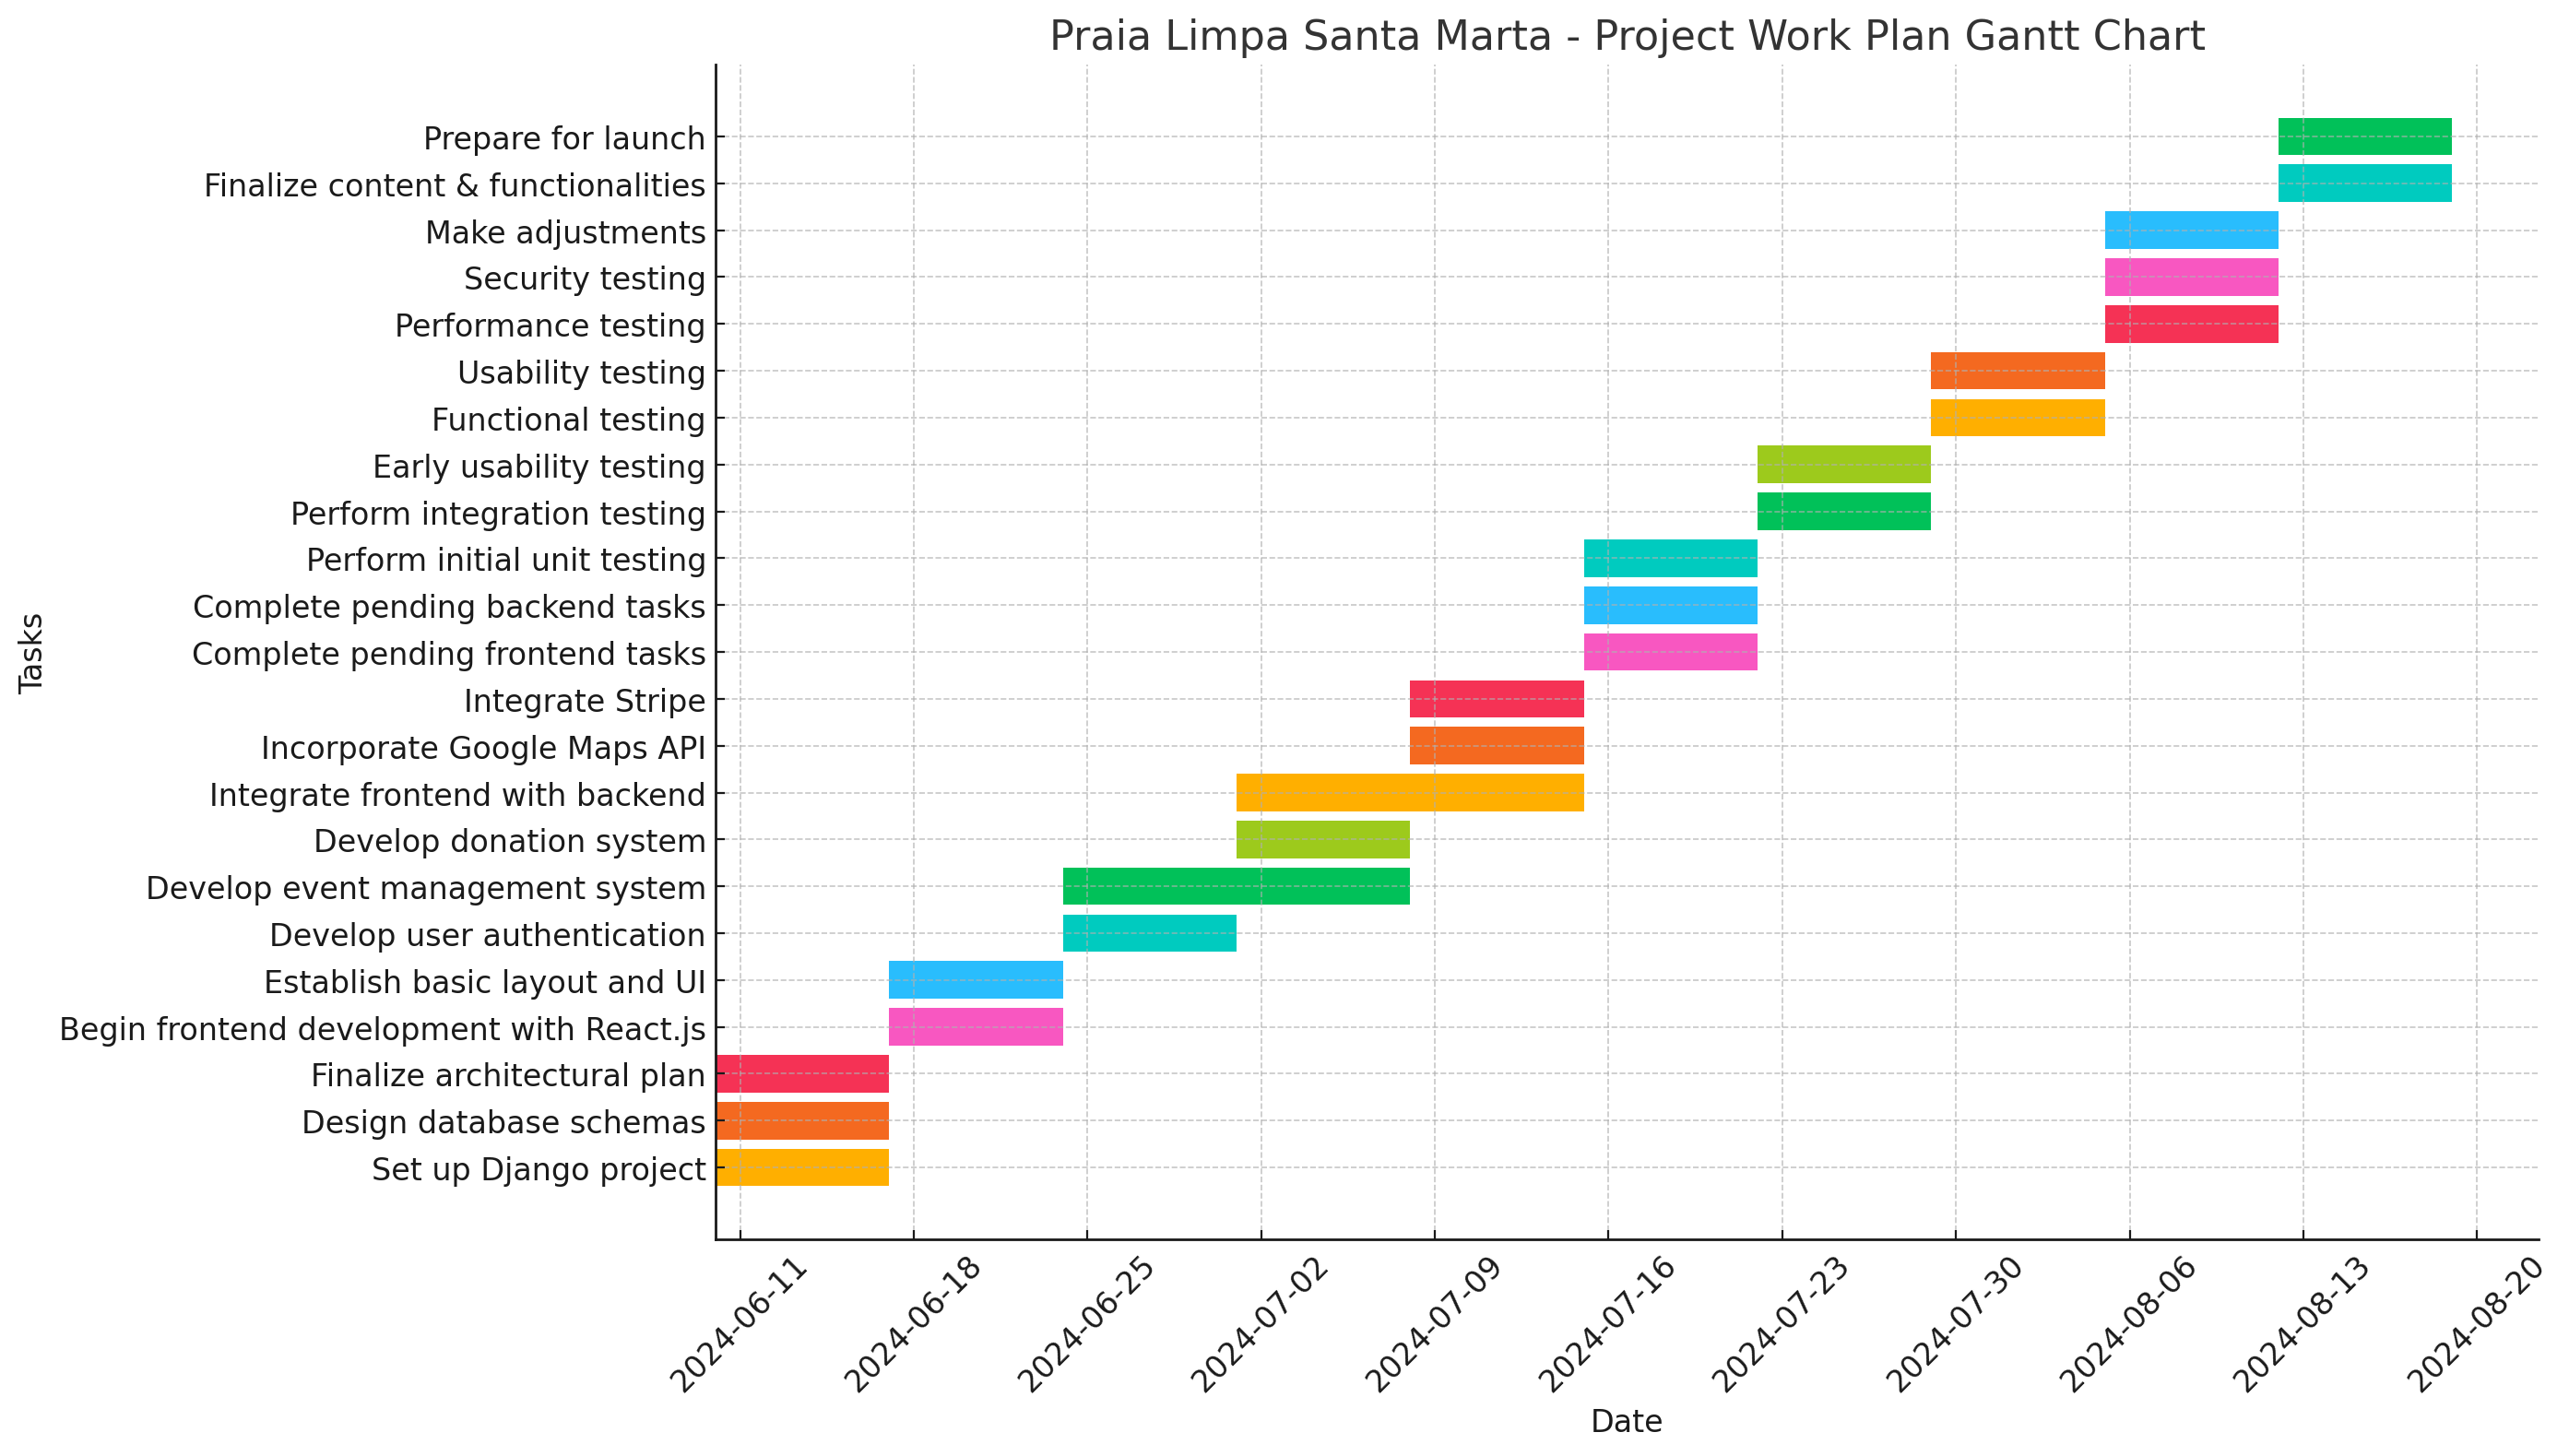
\includegraphics[width=1\textwidth]{images/gantt_chart.png}
    \caption{Project Work Plan}
    \label{fig:work_plan}
\end{figure}

\begin{itemize}
    \item \textbf{Phase 1 (Weeks 1-2):} Requirements Gathering and Initial Design
    \begin{itemize}
        \item Setting up the Django project, designing database schemas, and finalizing the project's architectural plan.
        \item Begin frontend development to establish the basic layout and user interface using HTML, CSS, and Bootstrap.
    \end{itemize}

    \item \textbf{Phase 2 (Weeks 3-5):} Core Development
    \begin{itemize}
        \item Development of the core backend features in Django, including user authentication, event management, and the donation system.
        \item Integration of the frontend with the backend to ensure seamless data flow and user experience.
        \item Begin incorporating external APIs such as Google Maps for event location services and Stripe for donation processing.
    \end{itemize}

    \item \textbf{Phase 3 (Weeks 6-7):} Feature Completion and Initial Testing
    \begin{itemize}
        \item Complete all pending frontend and backend development tasks.
        \item Perform initial unit and integration testing to identify and fix bugs.
        \item Start early usability testing with select community members to gather quick feedback.
    \end{itemize}

    \item \textbf{Phase 4 (Weeks 8-10):} Final Testing, Adjustments, and Launch Preparation
    \begin{itemize}
        \item Comprehensive testing phase, including functional, usability, performance, and security testing.
        \item Make necessary adjustments based on feedback from usability testing and test results.
        \item Finalize content, ensure all functionalities are polished, and prepare for project launch.
    \end{itemize}
\end{itemize}

\section{Kanban Ticketing System}

The development of the \textit{Farol de Santa Marta App} utilized the Kanban methodology\cite{kniberg2010}, a project management approach focused on continuous delivery and flexibility. This allowed the team to manage tasks visually while adapting to evolving requirements. A Kanban board was employed to organize tasks, providing transparency and efficient workflow management.

\subsection{Implementation of Kanban}

The Kanban board, managed using an online tool like monday.com\cite{monday}, was structured with the following columns:

\begin{itemize}
    \item \textbf{Not Started}: Tasks identified but not yet started, including setup, feature development, bug fixes, and documentation.
    \item \textbf{Working on It}: Ongoing tasks that provided visibility and ensured focus on active work.
    \item \textbf{Stuck}: Tasks facing obstacles, highlighting issues early and enabling timely resolution.
    \item \textbf{Done}: Completed tasks, showing progress and ensuring that all reviews and testing phases were passed.
\end{itemize}

\subsection{Application in Development Stages}

\begin{itemize}
    \item \textbf{Setup}: Initial tasks like configuring the Django framework and creating basic models were quickly moved through the board.
    \item \textbf{Feature Development}: Features such as courses, feedback, and the store were broken into smaller tasks and managed systematically through the Kanban system.
    \item \textbf{Bug Fixing}: Bugs and issues were tracked, ensuring timely fixes and project stability.
    \item \textbf{Documentation}: Final tasks related to documentation and deployment were managed through the board, ensuring no step was missed before project completion.
\end{itemize}

\begin{figure}[h]
    \centering
    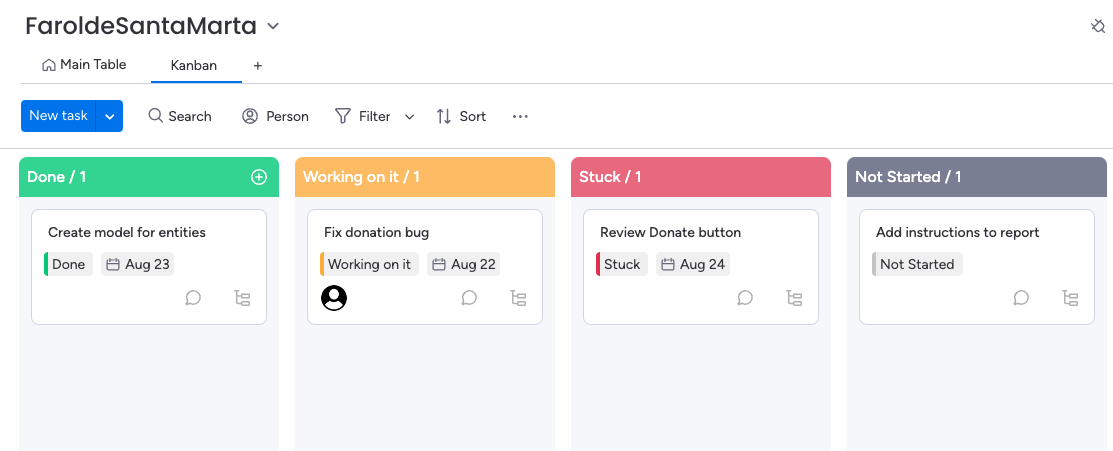
\includegraphics[width=0.8\textwidth]{images/kanban.png}
    \caption{Kanban Board Used in the Farol de Santa Marta App Development}
    \label{fig:kanban}
\end{figure}


%%% Local Variables:
%%% mode: latex
%%% TeX-master: "../../main"
%%% End:

\chapter{Implementation}
\label{ch:implementation}

% Choose your own headings.

\section{System architecture}

During the development phase, several challenges were encountered, notably the difficulty in identifying a suitable nonprofit organization to receive donations. This obstacle has influenced the project's direction and necessitated adjustments to the original plan.

Given more time, I intend to reach out to local community members to establish a nonprofit organization dedicated to the cause, fostering greater local involvement and ensuring compliance with regional laws and regulations.

As a result, the donation page remains under development, as it requires collaboration with local nonprofits to provide accurate information on how to receive donations and adhere to legal requirements. This delay has impacted the project's timeline and scope.

To create a more comprehensive and impactful platform, the decision was made to incorporate a login page that offers educational resources on environmental conservation. This addition allows students and community members to engage with the content, learn about sustainable practices, and contribute to the preservation of the local environment. This enhancement not only enriches the project but also aligns with its broader goals of fostering environmental awareness and action.

The Farol de Santa Marta website is designed with two primary components: an API that connects to a database to store information about environmental conservation activities, events, courses, and products, and a web application that serves both the general public and organizers. Visitors interested in environmental conservation can explore information on upcoming events, educational courses, and eco-friendly products provided through the API. Organizers can register and manage their events, courses, and even products in the online store.

The user journey begins with the login process, as illustrated in Diagram 1 made using Mermaid.js\cite{mermaid}. If a user does not have an account, they have the option to sign up. Once registered, the user can log in and be directed to the Dashboard. From the Dashboard, users can navigate through various sections such as "Events," "Courses," "Store," and "Get Involved." 

In the "Events" section, users can browse upcoming environmental conservation events. If no events match the user's selected criteria, a pop-up notification will alert them. If relevant events are available, a list will be presented, allowing the user to click on any event for more detailed information through a modal window.

In the "Courses" section, users can explore educational content on environmental conservation. Similar to the events, users can view detailed course information and enroll in courses that interest them.

The "Store" section offers eco-friendly products, where users can browse items, view details, and make purchases to support conservation efforts. 

This structure ensures that both participants and organizers have a smooth, intuitive experience, enabling them to engage fully with the environmental initiatives and offerings of Farol de Santa Marta.

\begin{figure}
    \centering
    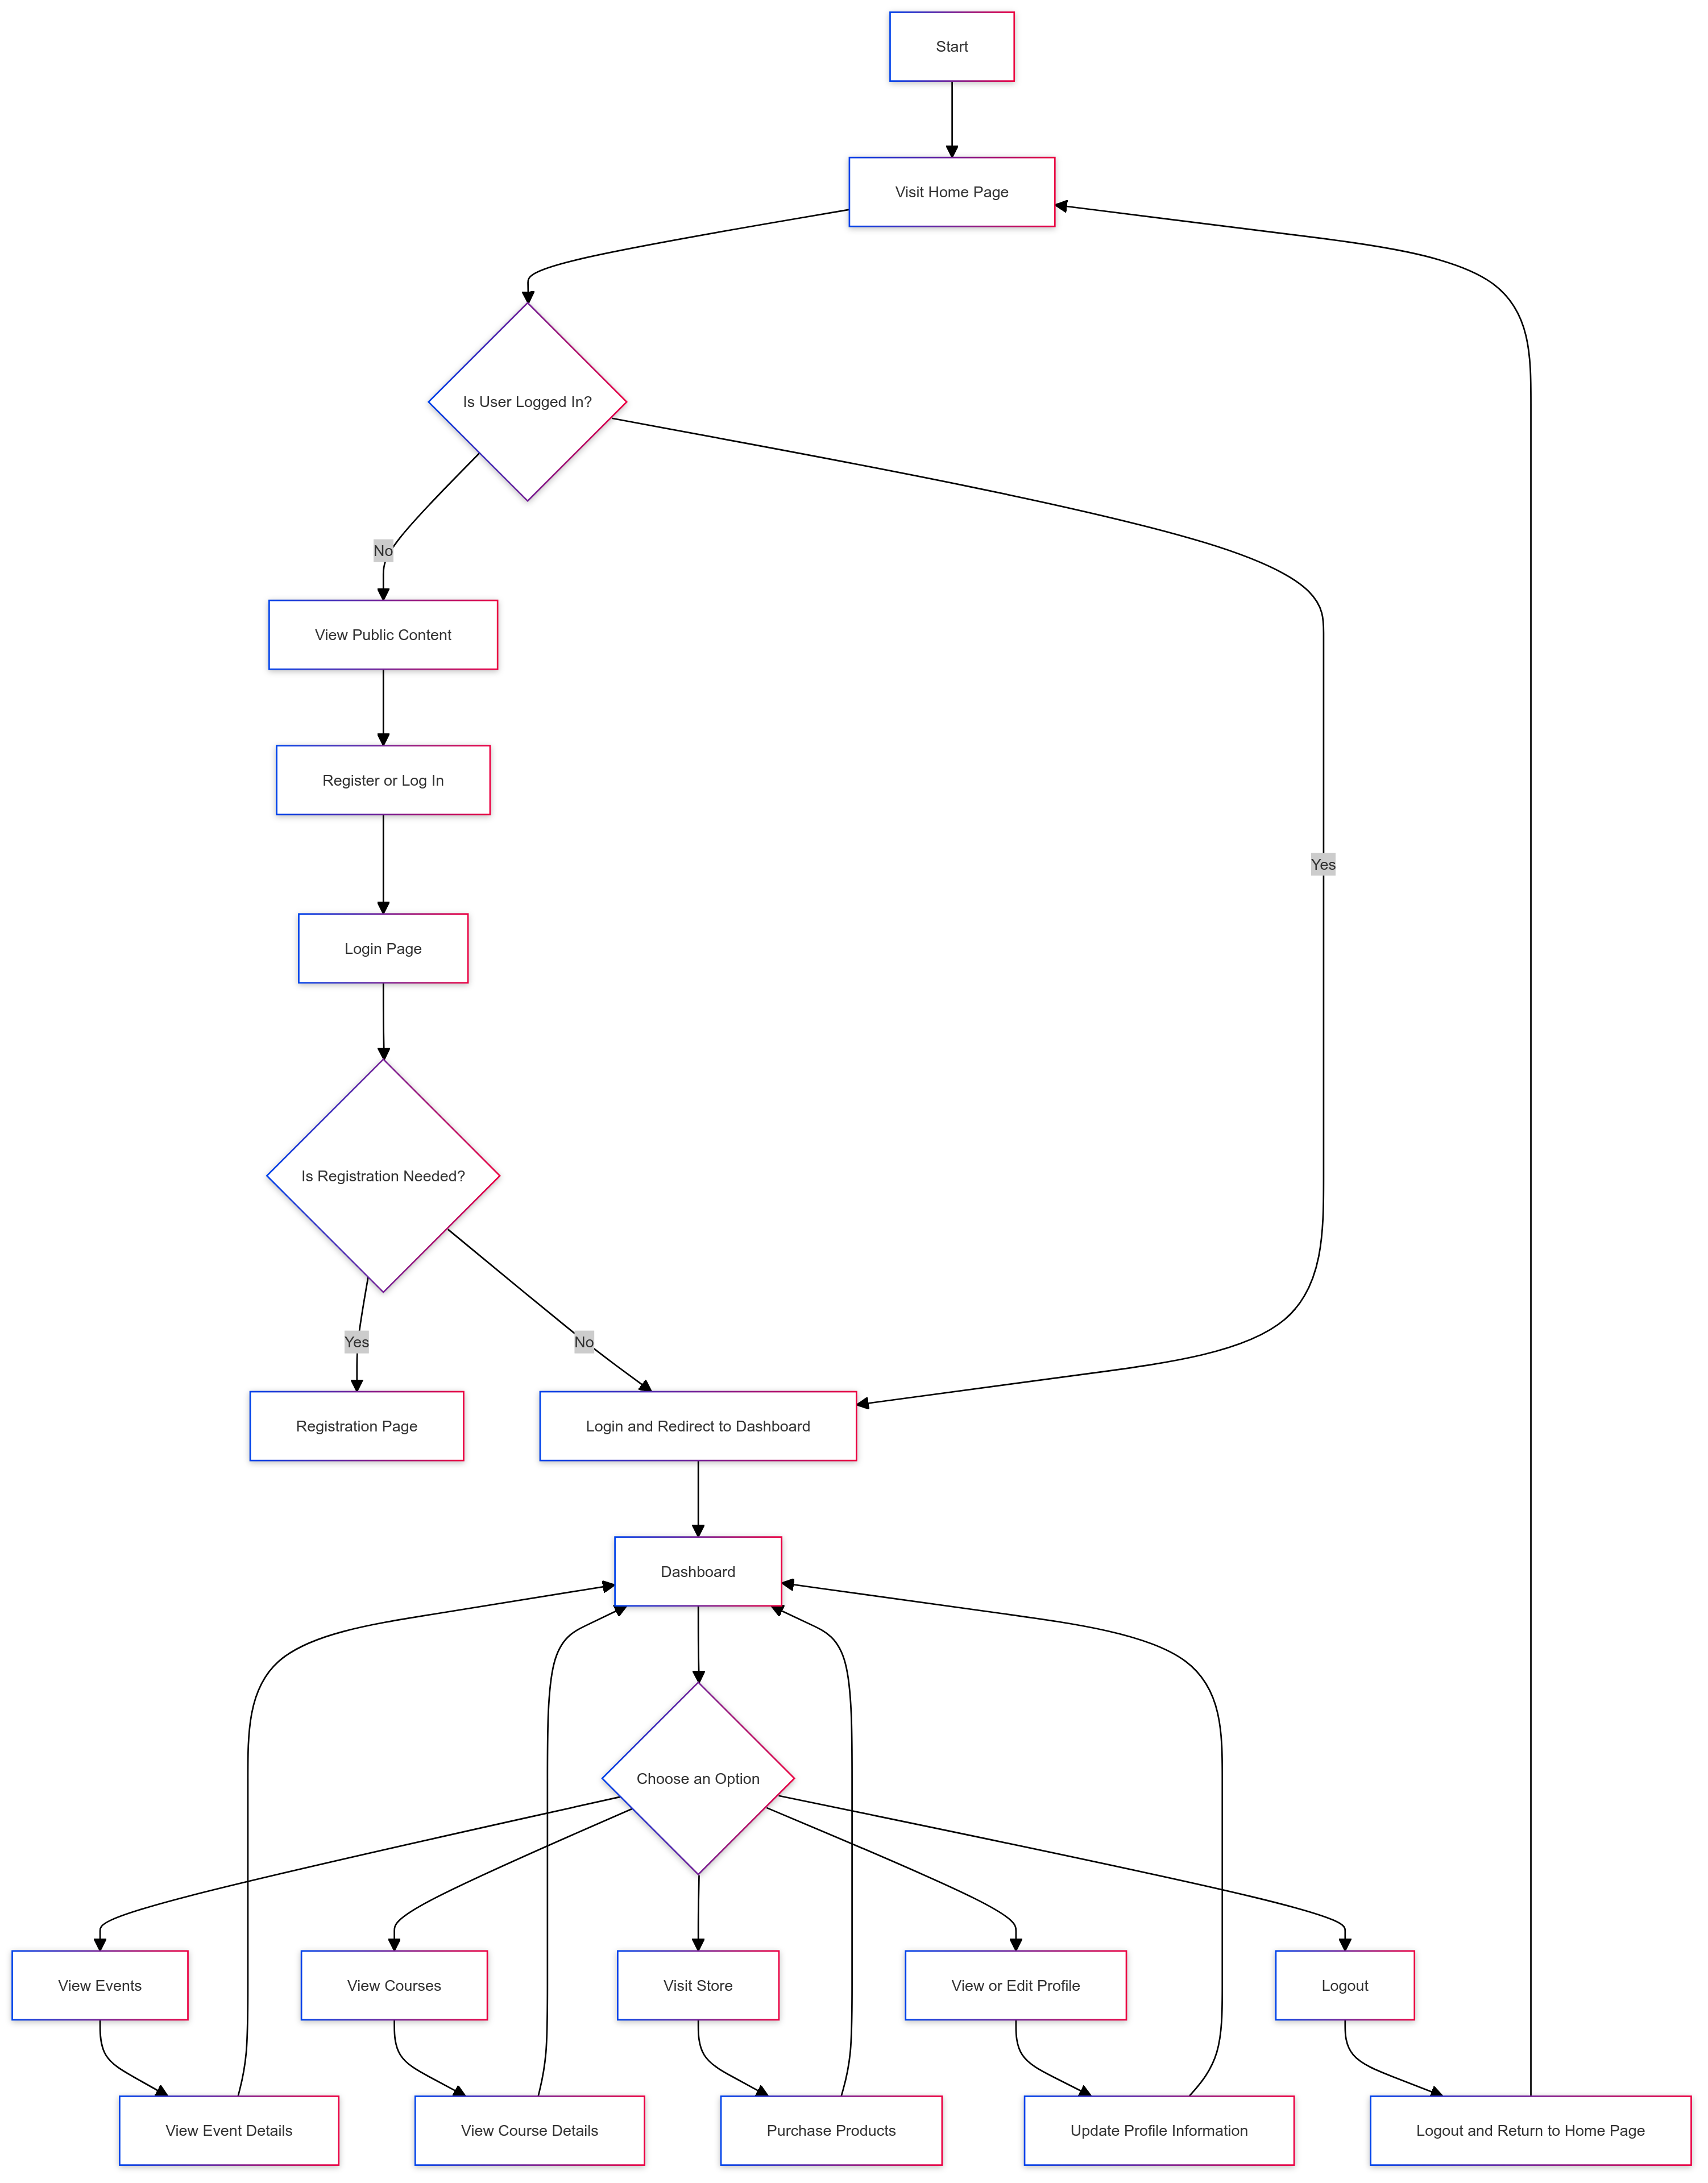
\includegraphics[width=1\linewidth]{images/mermaid-flow.png}
    \caption{Website Flowchart}
    \label{fig:Flowchart}
\end{figure}

\section{Software implementation}

The previous chapter presented the various technologies employed in the development of the Farol de Santa Marta website. This section delves deeper into the rationale behind the selection of these technologies and how each contributed to achieving the project’s goals.

Django, a high-level Python web framework, was chosen as the backbone of the website's backend. Its robust and scalable nature made it an ideal choice for managing the server-side logic of the application. Django’s built-in user authentication system allowed for secure user management, including login and registration functionalities. Furthermore, Django's ORM (Object-Relational Mapping) facilitated seamless interaction with the database, ensuring efficient data storage and retrieval operations.

SQLite was selected as the database solution for this project. As a lightweight, file-based database, SQLite was well-suited to the needs of this application, particularly given the project's scale. Its integration with Django is straightforward, allowing for quick setup and minimal configuration. SQLite's simplicity and reliability made it a fitting choice, ensuring that user data, events, courses, and other essential information could be managed efficiently.

On the front end, HTML5, CSS3, and JavaScript were used to structure, style, and add interactivity to the website. HTML5 provided a strong foundation for the markup, allowing for the creation of a semantically meaningful structure. CSS3 was utilized to ensure that the visual presentation of the website was both modern and responsive, making it accessible across various devices and screen sizes. JavaScript added the necessary interactivity, enabling dynamic user experiences that enhance engagement and usability.

Bootstrap was employed as the front-end framework to expedite the design process. Known for its responsive grid system and pre-built components, Bootstrap enabled the rapid development of a visually appealing and consistent user interface. This was particularly important for ensuring that the website could be accessed easily on different devices, providing a seamless experience whether users were on a desktop, tablet, or smartphone.

Mermaid.js was integrated into the project documentation to create diagrams and flowcharts that visually represent the system architecture and user navigation flows. This tool proved invaluable for communicating complex structures and processes clearly, making it easier for developers and stakeholders to understand the website’s design and functionality.

Finally, although still under development, the donation page will incorporate Stripe or a similar payment gateway. This technology was chosen for its reputation in handling secure online transactions, which is crucial for processing donations. Stripe's robust API and compliance with global financial regulations make it a reliable choice for ensuring that all transactions are processed securely and in accordance with legal requirements.

\section*{Intended Users}

The Farol de Santa Marta website is designed to serve a diverse audience, each with specific needs and motivations related to environmental conservation.

The primary user group consists of \textbf{local community members}, who are residents of Farol de Santa Marta and surrounding areas. These users are deeply invested in preserving their local environment and will utilize the website to stay informed about upcoming conservation events, participate in activities such as beach clean-ups, and access educational resources. Their primary motivation is to contribute to the preservation of their home, ensuring that the natural beauty of Farol de Santa Marta is maintained for future generations.

Another significant user group includes \textbf{tourists}, both domestic and international, who visit the region to enjoy its scenic beaches and natural attractions. These users seek information on local conservation practices and opportunities to engage in eco-friendly activities during their stay. They are motivated by a desire to enjoy the natural beauty of the area while minimizing their environmental impact, in line with the growing trend of sustainable tourism.

\textbf{Environmental activists and volunteers} also represent a key demographic for the website. These individuals are passionate about conservation and may or may not be local to the area. They will use the platform to find volunteer opportunities, make donations, and connect with like-minded individuals and organizations. Their motivation is driven by a strong commitment to sustainability and the desire to take actionable steps to protect the environment.

The website also targets \textbf{students and educators} interested in environmental studies, particularly those focused on marine and coastal ecosystems. Students will use the platform to enroll in educational courses, while educators may contribute content or use the site as a teaching tool. Their motivation lies in gaining and imparting knowledge about environmental conservation, with a focus on practical, community-based approaches.

Additionally, the website is intended for \textbf{nonprofit organizations and partners} involved in or supporting conservation efforts in the region. These organizations will use the platform to collaborate on projects, promote events, and connect with volunteers and donors. Their motivation is to expand their impact by engaging with a broader audience and securing resources for their initiatives.

\textbf{Donors}, who are individuals and entities interested in financially supporting environmental conservation in Farol de Santa Marta, will also find the website useful. They seek transparency regarding the use of their contributions and the impact of their donations. Their motivation is to support environmental causes and ensure that their financial contributions are making a tangible difference.

Finally, the website will be managed by \textbf{website administrators}, who are responsible for maintaining and updating the site. These users need tools to efficiently manage content, user roles, and technical operations, ensuring the website's smooth operation and its ability to meet the needs of its diverse user base.

\newpage
\section*{Functional Requirements for the Farol de Santa Marta App}

\begin{longtable}{|>{\raggedright}m{2cm}|>{\raggedright}m{4cm}|>{\raggedright\arraybackslash}m{8cm}|}
\hline
\textbf{Identifier} & \textbf{Functional Requirement} & \textbf{Detailed Description} \\
\hline
RF-01 & User Registration & The user must have the ability to register in the system by providing information such as name, email, and password. \\
\hline
RF-02 & User Authentication & The user must have the ability to log in to the system using their credentials. \\
\hline
RF-03 & Course Enrollment & The student user must have the ability to enroll in environmental conservation courses available on the platform. \\
\hline
RF-04 & Course Creation & The teacher user must have the ability to create and manage courses, including adding descriptions and course materials. \\
\hline
RF-05 & Course Viewing & The user must have the ability to view a list of available courses and their details. \\
\hline
RF-06 & Course Feedback & The user must have the ability to leave feedback on courses they have participated in, including comments and ratings. \\
\hline
RF-07 & Product Purchase & The user must have the ability to purchase eco-friendly products from the platform's store. \\
\hline
RF-08 & Donations & The user must have the ability to make donations to support environmental conservation projects through the system. \\
\hline
RF-09 & Event Viewing & The user must have the ability to view environmental conservation events organized in the region. \\
\hline
RF-10 & User Logout & The user must have the ability to log out of the system to end their session. \\
\hline
\end{longtable}

\subsection*{Explanation of the Columns}

\begin{itemize}
    \item \textbf{Identifier}: The unique code assigned to each functional requirement.
    \item \textbf{Functional Requirement}: The name or title of the requirement.
    \item \textbf{Detailed Description}: A detailed explanation of what the functional requirement should accomplish within the system.
\end{itemize}

This table of functional requirements serves as a guide for development, ensuring that all key functionalities of the \textbf{Farol de Santa Marta App} are implemented as planned.

\section{Data Model and Attributes}

This section presents the data model used for the \textit{Farol de Santa Marta} application. The model is represented by an Entity-Relationship Diagram (ERD) that defines the entities, their attributes, and the relationships between them.

\subsection{Entities and Attributes}

The application model and attributes are described as the Figure shows:
\begin{figure}
    \centering
    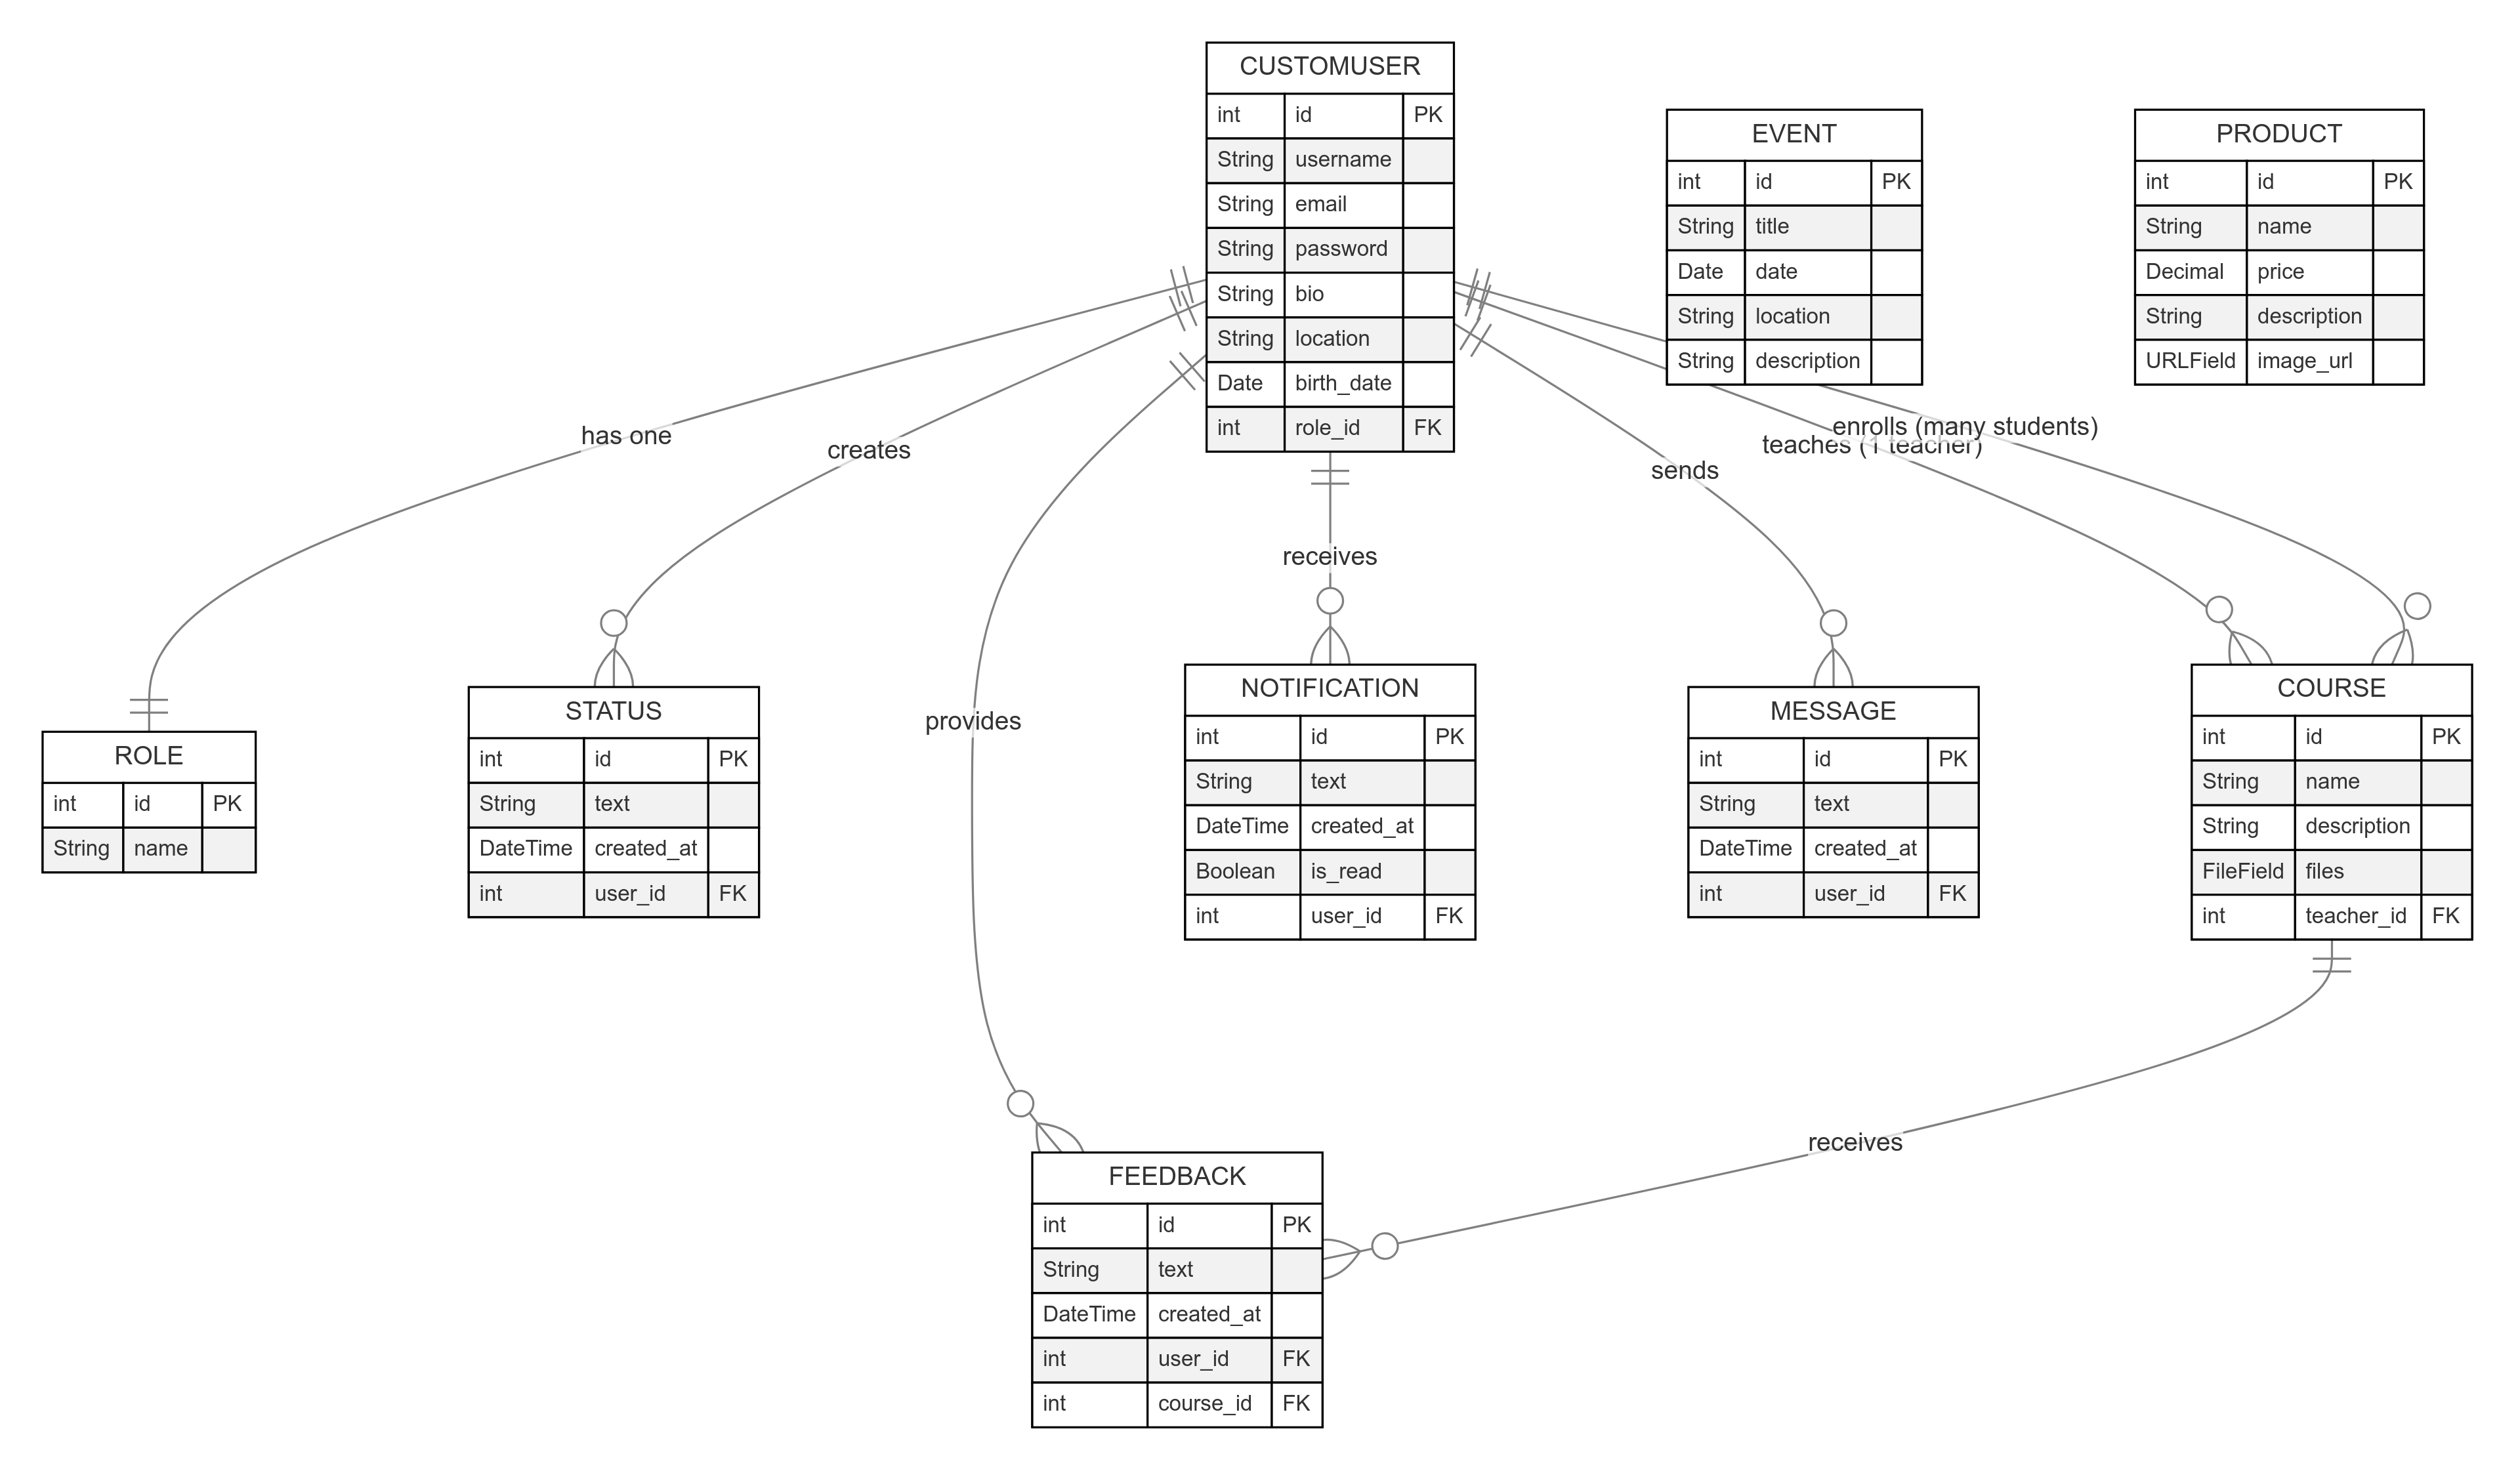
\includegraphics[width=1\linewidth]{images/er-diagram.png}
    \caption{ER Diagram}
    \label{fig:ER Diagram}
\end{figure}

\begin{itemize}
    \item \textbf{CUSTOMUSER}: The \texttt{CUSTOMUSER} entity represents the users of the system. Each user has the following attributes:
    \begin{itemize}
        \item \textbf{id (PK)}: A unique identifier for each user (Primary Key).
        \item \textbf{username}: The user's chosen name for logging into the system.
        \item \textbf{email}: The user's email address, used for communication and login purposes.
        \item \textbf{password}: The encrypted password for the user’s account.
        \item \textbf{bio}: A brief biography or description provided by the user.
        \item \textbf{location}: The user's location, which can be a city, state, or country.
        \item \textbf{birth\_date}: The user's birth date.
        \item \textbf{role\_id (FK)}: A foreign key linking the user to a specific role, enforcing the rule that each user can have only one role.
    \end{itemize}

    \item \textbf{ROLE}: The \texttt{ROLE} entity defines the different roles a user can have in the system. Each role has:
    \begin{itemize}
        \item \textbf{id (PK)}: A unique identifier for each role (Primary Key).
        \item \textbf{name}: The name of the role (e.g., "Student", "Teacher").
    \end{itemize}

    \item \textbf{STATUS}: The \texttt{STATUS} entity represents status updates posted by users. Attributes include:
    \begin{itemize}
        \item \textbf{id (PK)}: A unique identifier for each status update (Primary Key).
        \item \textbf{text}: The content of the status update.
        \item \textbf{created\_at}: The timestamp of when the status was created.
        \item \textbf{user\_id (FK)}: A foreign key linking the status to a specific user.
    \end{itemize}

    \item \textbf{COURSE}: The \texttt{COURSE} entity represents the courses offered in the system. Each course has:
    \begin{itemize}
        \item \textbf{id (PK)}: A unique identifier for each course (Primary Key).
        \item \textbf{name}: The name of the course.
        \item \textbf{description}: A brief description of what the course entails.
        \item \textbf{files}: A field for uploading course-related files (e.g., PDFs, documents).
        \item \textbf{teacher\_id (FK)}: A foreign key linking the course to the teacher who created it.
    \end{itemize}

    \item \textbf{FEEDBACK}: The \texttt{FEEDBACK} entity captures feedback provided by users on specific courses. Attributes include:
    \begin{itemize}
        \item \textbf{id (PK)}: A unique identifier for each feedback entry (Primary Key).
        \item \textbf{text}: The content of the feedback.
        \item \textbf{created\_at}: The timestamp of when the feedback was provided.
        \item \textbf{user\_id (FK)}: A foreign key linking the feedback to the user who provided it.
        \item \textbf{course\_id (FK)}: A foreign key linking the feedback to the specific course it relates to.
    \end{itemize}

    \item \textbf{NOTIFICATION}: The \texttt{NOTIFICATION} entity represents notifications sent to users. Each notification has:
    \begin{itemize}
        \item \textbf{id (PK)}: A unique identifier for each notification (Primary Key).
        \item \textbf{text}: The content of the notification.
        \item \textbf{created\_at}: The timestamp of when the notification was created.
        \item \textbf{is\_read}: A boolean value indicating whether the notification has been read.
        \item \textbf{user\_id (FK)}: A foreign key linking the notification to a specific user.
    \end{itemize}

    \item \textbf{MESSAGE}: The \texttt{MESSAGE} entity stores messages sent by users. Attributes include:
    \begin{itemize}
        \item \textbf{id (PK)}: A unique identifier for each message (Primary Key).
        \item \textbf{text}: The content of the message.
        \item \textbf{created\_at}: The timestamp of when the message was sent.
        \item \textbf{user\_id (FK)}: A foreign key linking the message to the user who sent it.
    \end{itemize}

    \item \textbf{EVENT}: The \texttt{EVENT} entity represents events related to environmental conservation activities. Each event has:
    \begin{itemize}
        \item \textbf{id (PK)}: A unique identifier for each event (Primary Key).
        \item \textbf{title}: The title or name of the event.
        \item \textbf{date}: The date when the event is scheduled to occur.
        \item \textbf{location}: The location where the event will take place.
        \item \textbf{description}: A detailed description of the event.
    \end{itemize}

    \item \textbf{PRODUCT}: The \texttt{PRODUCT} entity represents items available for purchase in the system’s store. Each product has:
    \begin{itemize}
        \item \textbf{id (PK)}: A unique identifier for each product (Primary Key).
        \item \textbf{name}: The name of the product.
        \item \textbf{price}: The cost of the product, represented as a decimal value.
        \item \textbf{description}: A detailed description of the product.
        \item \textbf{image\_url}: A URL linking to an image of the product.
    \end{itemize}
\end{itemize}

\subsection{Relationships Between Entities}

\begin{itemize}
    \item \textbf{CUSTOMUSER and ROLE}: The relationship between \texttt{CUSTOMUSER} and \texttt{ROLE} is one-to-one, meaning each user can only have one role at a time.

    \item \textbf{CUSTOMUSER and STATUS}: A one-to-many relationship, where a user can create multiple status updates.

    \item \textbf{CUSTOMUSER and NOTIFICATION}: A one-to-many relationship, where a user can receive multiple notifications.

    \item \textbf{CUSTOMUSER and MESSAGE}: A one-to-many relationship, where a user can send multiple messages.

    \item \textbf{CUSTOMUSER and FEEDBACK}: A one-to-many relationship, where a user can provide feedback for multiple courses.

    \item \textbf{COURSE and FEEDBACK}: A one-to-many relationship, where a course can receive multiple feedback entries.

    \item \textbf{CUSTOMUSER and COURSE}:
    \begin{itemize}
        \item \textbf{Teacher Relationship}: A one-to-many relationship, where a teacher can create and manage multiple courses.
        \item \textbf{Student Relationship}: A many-to-many relationship, where multiple students can enroll in multiple courses.
    \end{itemize}
\end{itemize}

\section{Prototyping}

The design of the \textit{Farol de Santa Marta} website was heavily inspired by the best practices and successful strategies observed during the research phase. The initial prototype was developed with a strong emphasis on usability, accessibility, and visual appeal, drawing from the elements that were identified as effective in engaging users and promoting environmental causes.

\subsection{Inspiration from Existing Websites}

During the research phase, several websites were analyzed to understand how they effectively communicate their missions, engage with their audience, and drive user actions such as donations, volunteer sign-ups, and participation in educational activities. Key websites that influenced the design include:

\begin{itemize}
    \item \textbf{Charity: Water}: Known for its clean, visually striking interface and impactful use of imagery, \textit{Charity: Water} provided inspiration for the visual design of the \textit{Farol de Santa Marta} website. The use of high-quality images, clear typography, and a straightforward layout were key elements adopted from this site.

    \item \textbf{World Wildlife Fund (WWF)}: The \textit{WWF} website's effective use of concise messaging and strategic placement of calls-to-action (CTAs) influenced the placement and design of similar elements on the \textit{Farol de Santa Marta} platform. The emphasis on highlighting the impact of user contributions through powerful visuals and succinct text was a direct inspiration for the prototype.

    \item \textbf{Greenpeace}: The \textit{Greenpeace} website's focus on activism and community engagement provided valuable insights into designing interactive elements, such as the "Get Involved" section, which encourages users to participate in local conservation activities. The prototype incorporated similar engagement strategies to foster a sense of community and collective responsibility among users.
\end{itemize}

\section{Overview of Key Pages}

This chapter presents the implemented and operational application, in accordance with the functional and non-functional requirements of the system. It provides a detailed overview of the development of each feature and component. The implementation will be showcased in desktop mode.

\subsection{Home page}

The homepage of the Farol de Santa Marta website serves as the central hub for users, offering a welcoming and visually appealing introduction to the platform. Designed with both aesthetics and functionality in mind, the homepage features a prominent hero section with a background image that captures the natural beauty of the coastline, immediately engaging visitors. The page is structured to provide easy navigation, with clear calls-to-action that guide users to key sections such as events, courses, and ways to get involved in environmental conservation efforts. By combining responsive design elements with compelling content, the homepage effectively communicates the mission of Farol de Santa Marta and invites users to explore and participate in the community's efforts to preserve the local environment.

\begin{figure}[H]
    \centering
    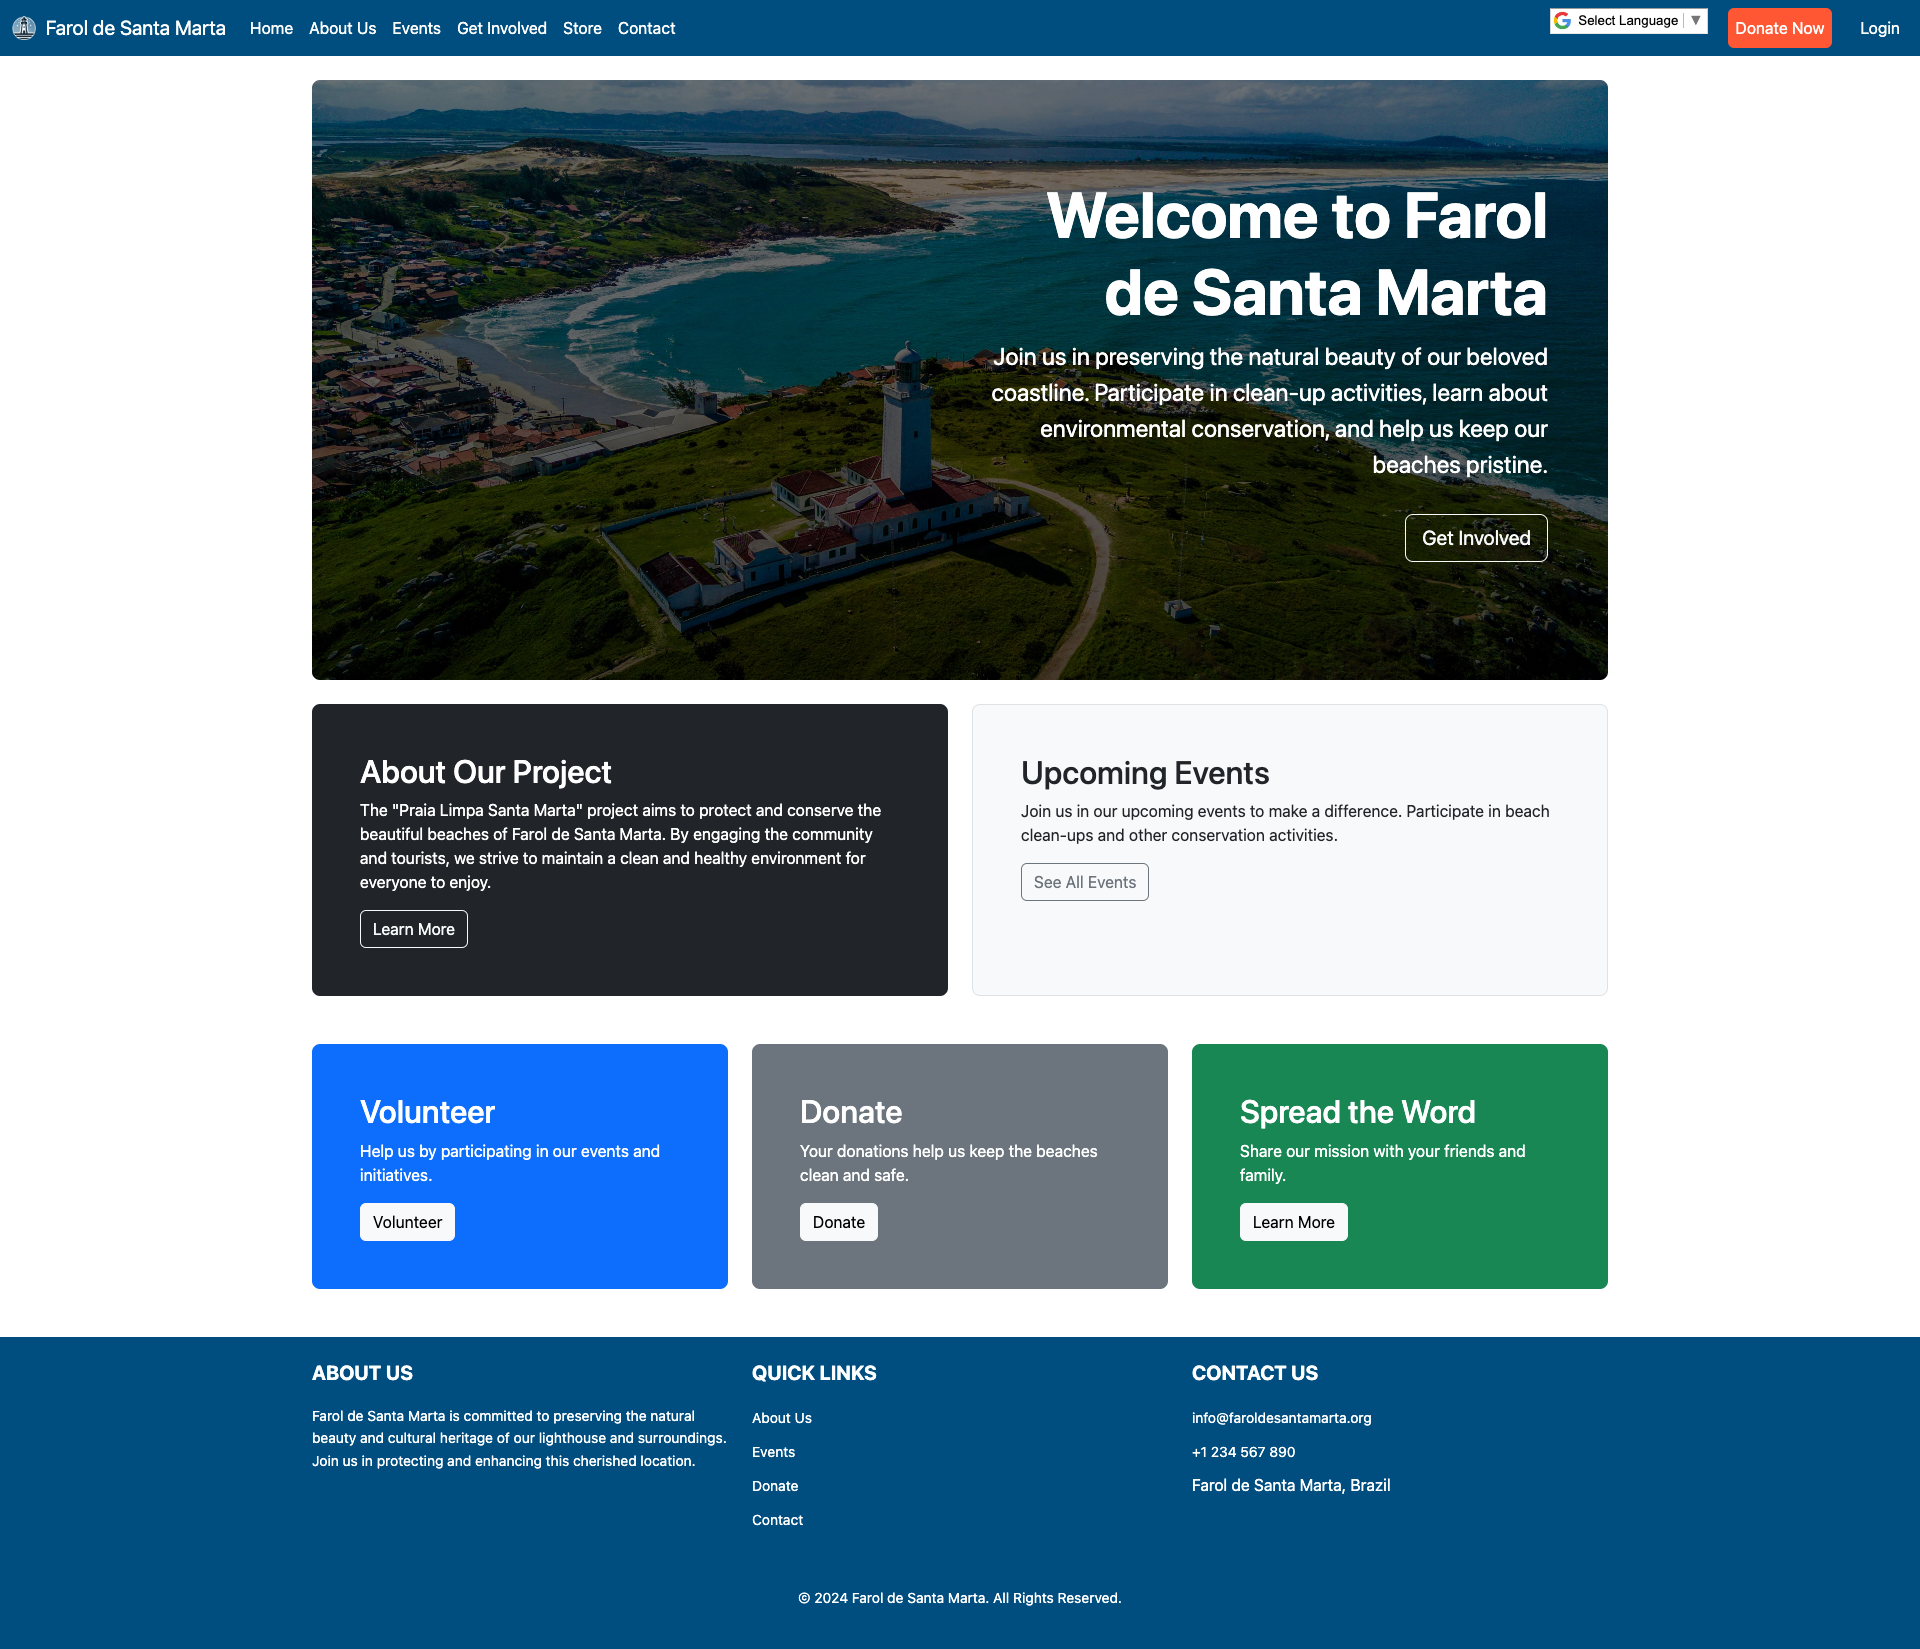
\includegraphics[width=1\linewidth]{images/home-page.png}
    \caption{Home page}
    \label{fig:Home page}
\end{figure}

\subsection{Events Page}

The \textbf{Events Page} serves as a central location for users to discover and participate in upcoming environmental conservation activities. It lists all the scheduled events, such as beach clean-ups and educational workshops, along with details including the date, location, and a brief description of each event. Users can easily browse through the events, click for more details, and sign up to participate, fostering community involvement in local conservation efforts.

\begin{figure}[H]
    \centering
    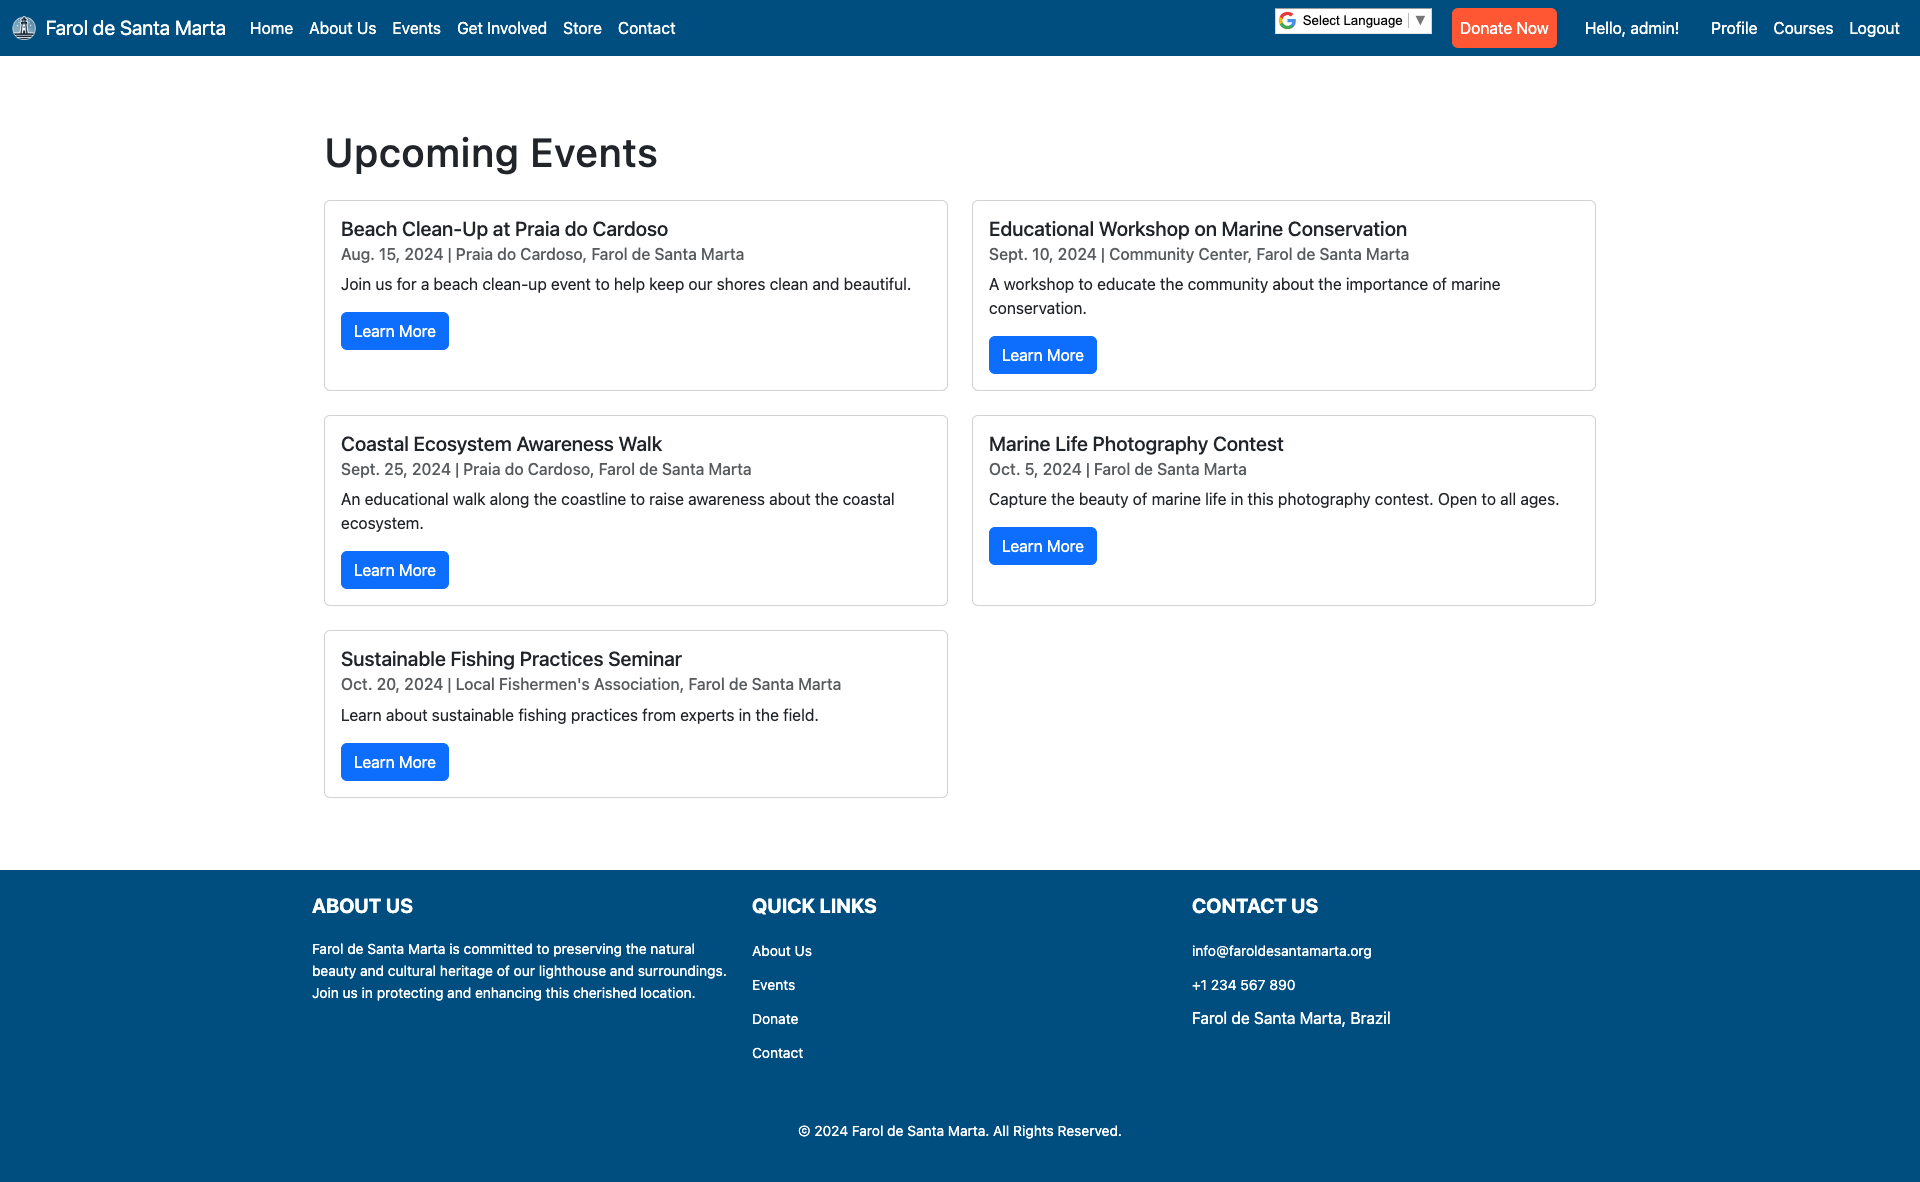
\includegraphics[width=\textwidth]{images/events-page.png}
    \caption{Example of the Events Page}
    \label{fig:events_page}
\end{figure}

\subsection{Donate Page}

The \textbf{Donate Page} is designed to facilitate financial contributions to support the ongoing conservation initiatives of \textit{Farol de Santa Marta}. The page offers a streamlined donation process, allowing users to select a predefined amount or enter a custom donation. Secure payment processing is integrated, ensuring that contributions are handled safely. The page also provides information on how donations are used, reinforcing transparency and encouraging user trust and generosity.

\begin{figure}[H]
    \centering
    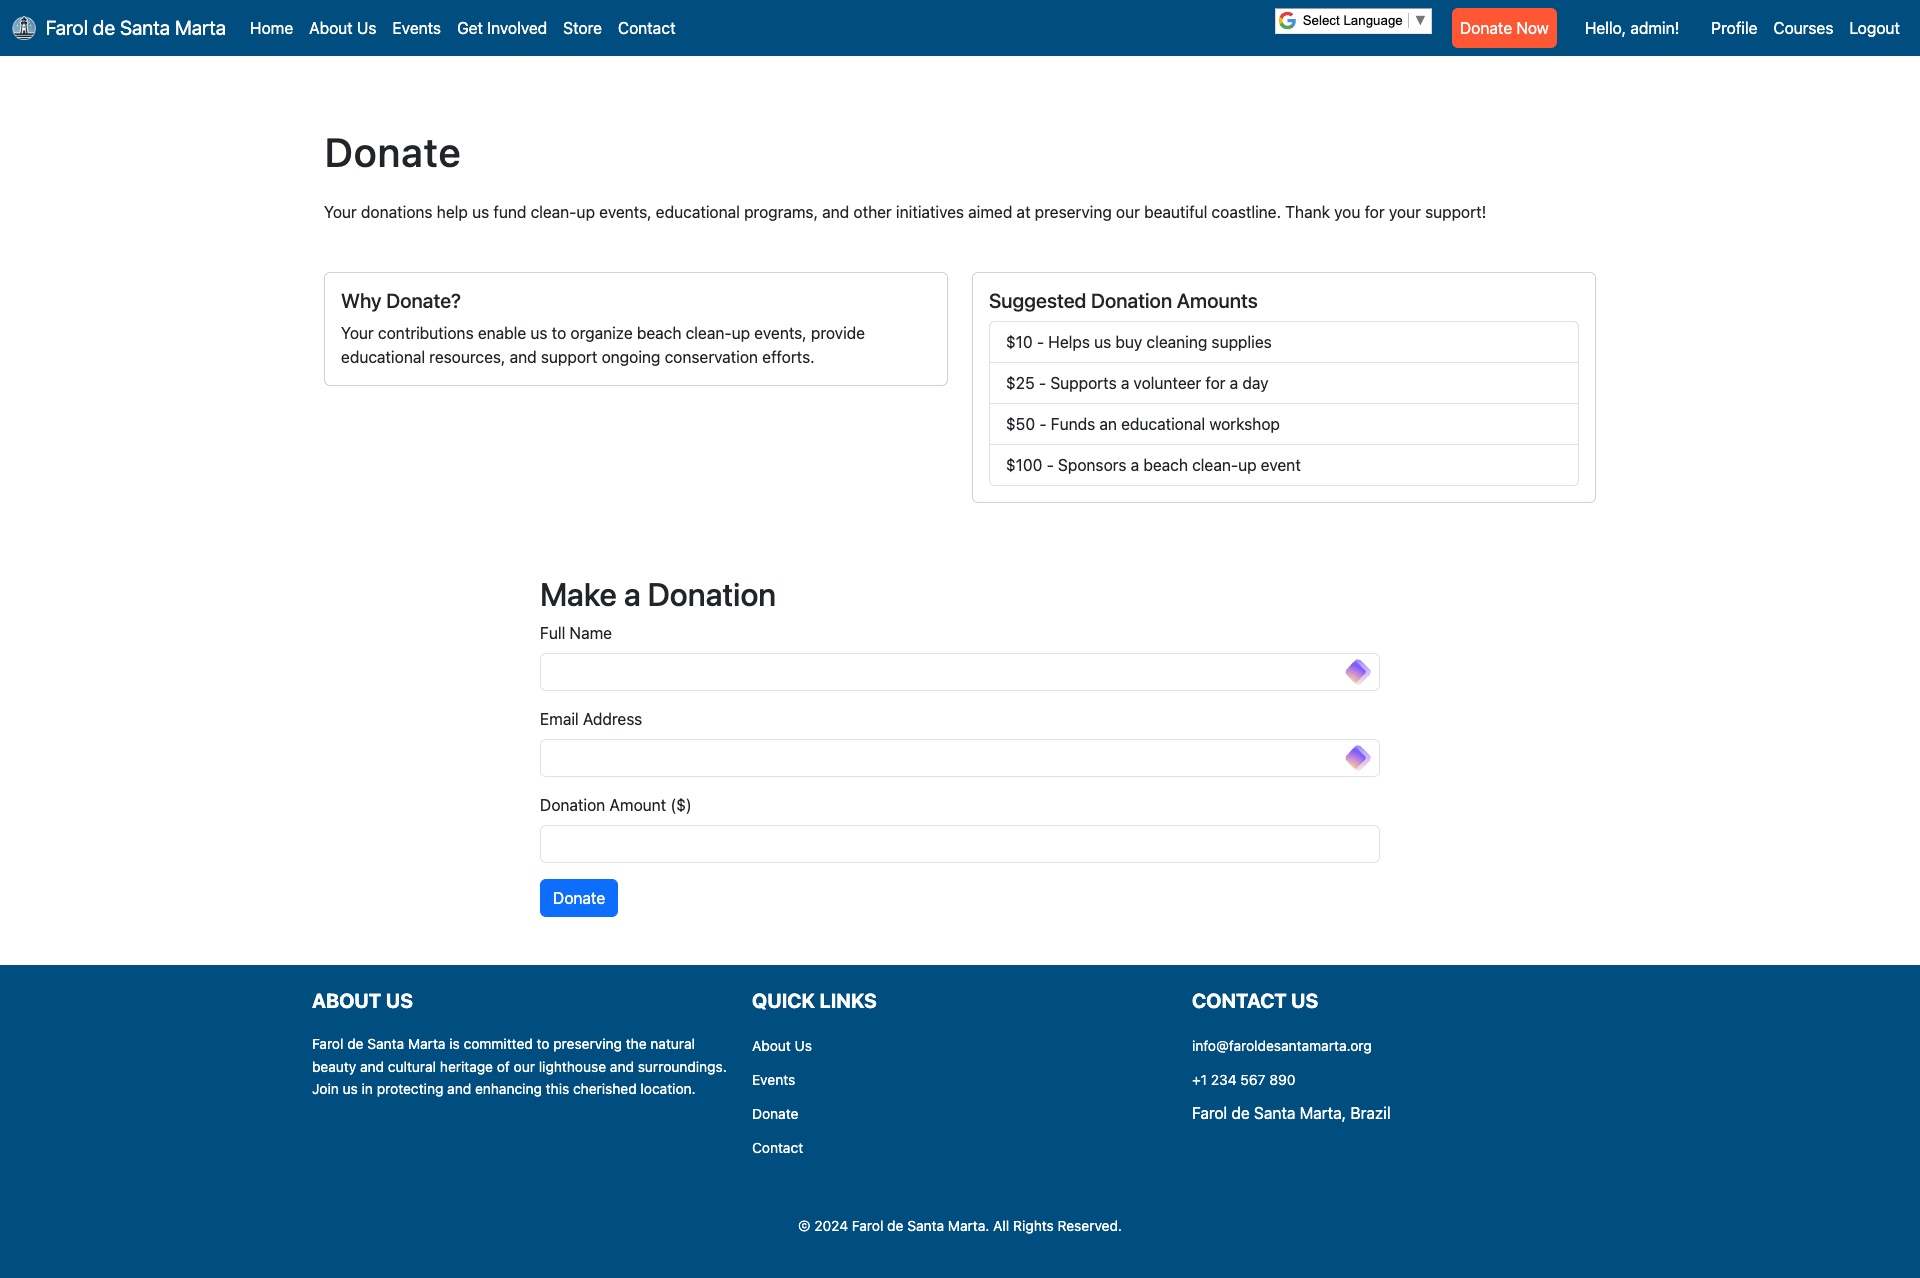
\includegraphics[width=\textwidth]{images/donate-page.png}
    \caption{Example of the Donate Page}
    \label{fig:donate_page}
\end{figure}

\subsection{Store Page}

The \textbf{Store Page} offers users the opportunity to purchase eco-friendly products, with all proceeds supporting the environmental initiatives of the organization. The store features items such as reusable water bottles, tote bags, and other sustainable goods, each accompanied by a description, price, and product image. This page not only serves as a fundraising tool but also promotes sustainable living by offering environmentally responsible products.

\begin{figure}[H]
    \centering
    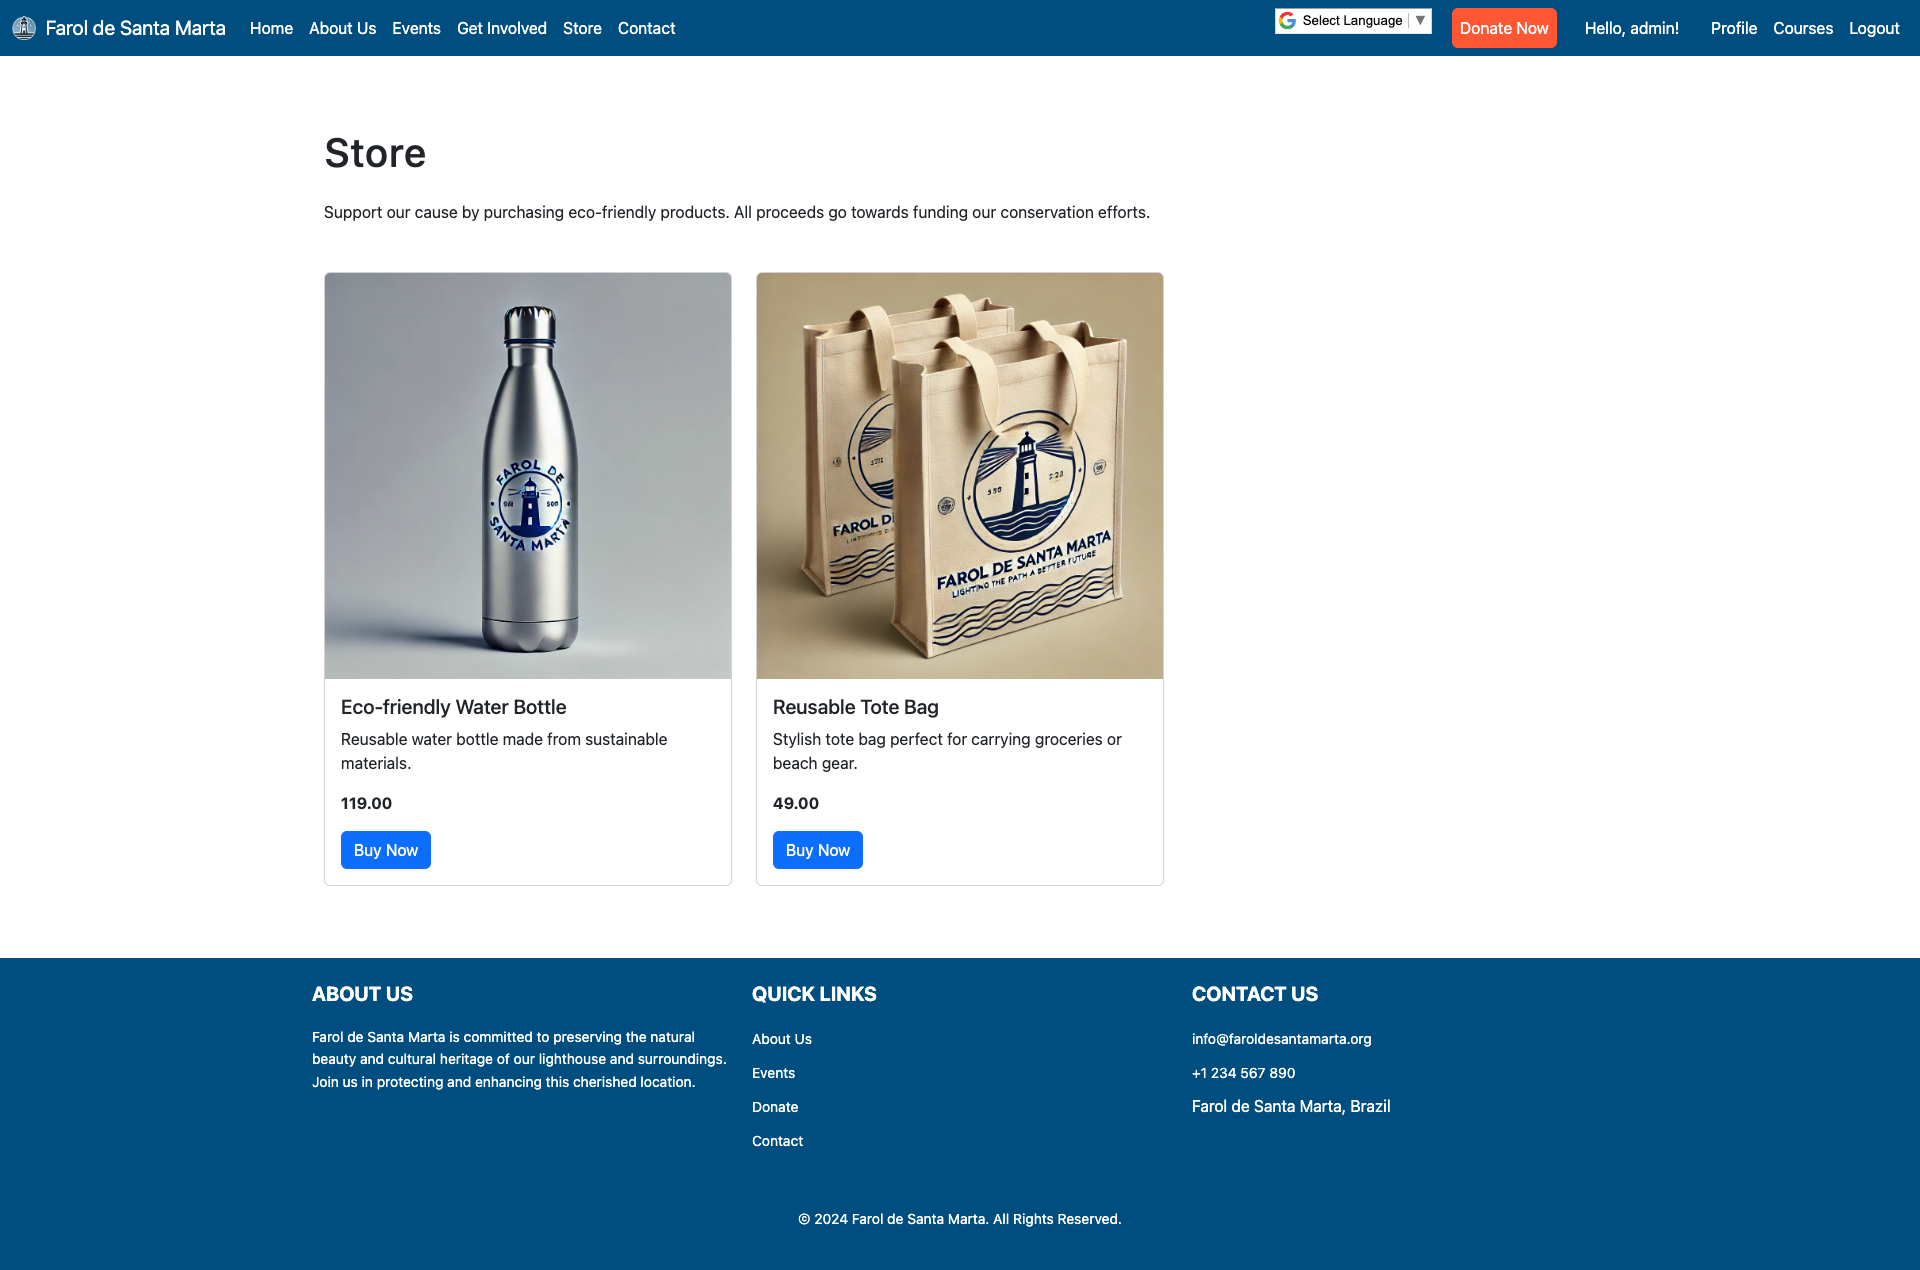
\includegraphics[width=\textwidth]{images/store-page.png}
    \caption{Example of the Store Page}
    \label{fig:store_page}
\end{figure}

\subsection{Courses Page}

The \textbf{Courses Page} provides access to educational resources focused on environmental conservation. Users, particularly students, can browse and enroll in various courses designed to enhance their understanding of sustainable practices and local environmental issues. Each course listing includes a description, instructor information, and any associated materials, fostering a learning environment that supports the mission of \textit{Farol de Santa Marta}.

\begin{figure}[H]
    \centering
    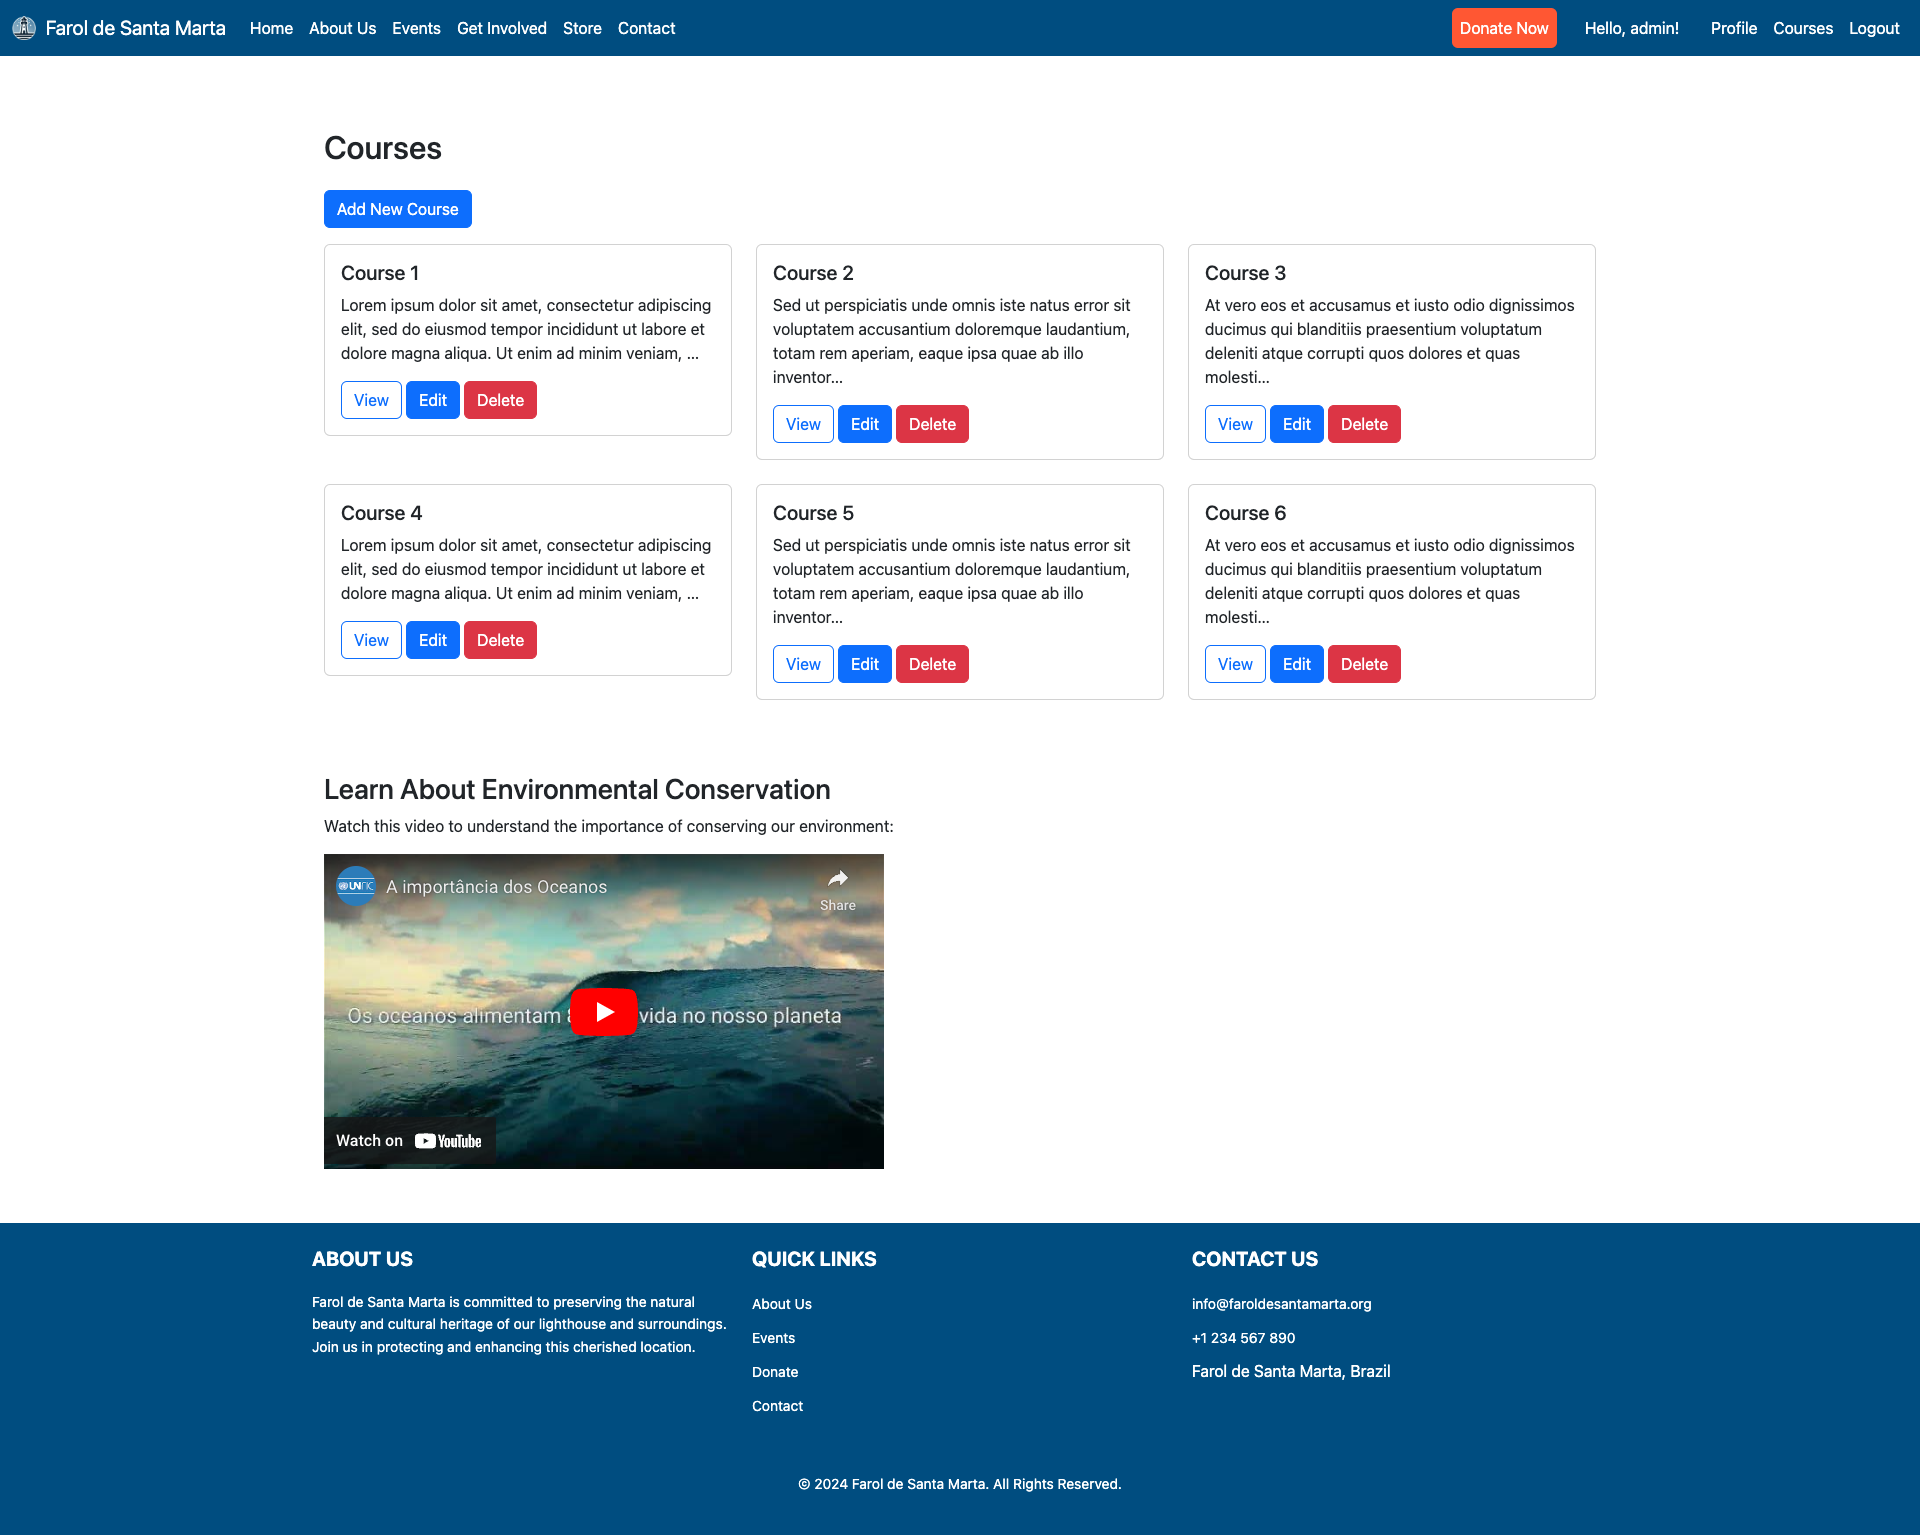
\includegraphics[width=\textwidth]{images/courses-page.png}
    \caption{Example of the Courses Page}
    \label{fig:courses_page}
\end{figure}

\subsection{Register Page}

The \textbf{Register Page} is the entry point for new users wishing to join the \textit{Farol de Santa Marta} community. It offers a straightforward registration process where users can create an account by providing essential information such as their name, email, and password. Upon successful registration, users gain access to additional features of the site, including event sign-ups, course enrollment, and the ability to make donations or purchases from the store.

\begin{figure}[H]
    \centering
    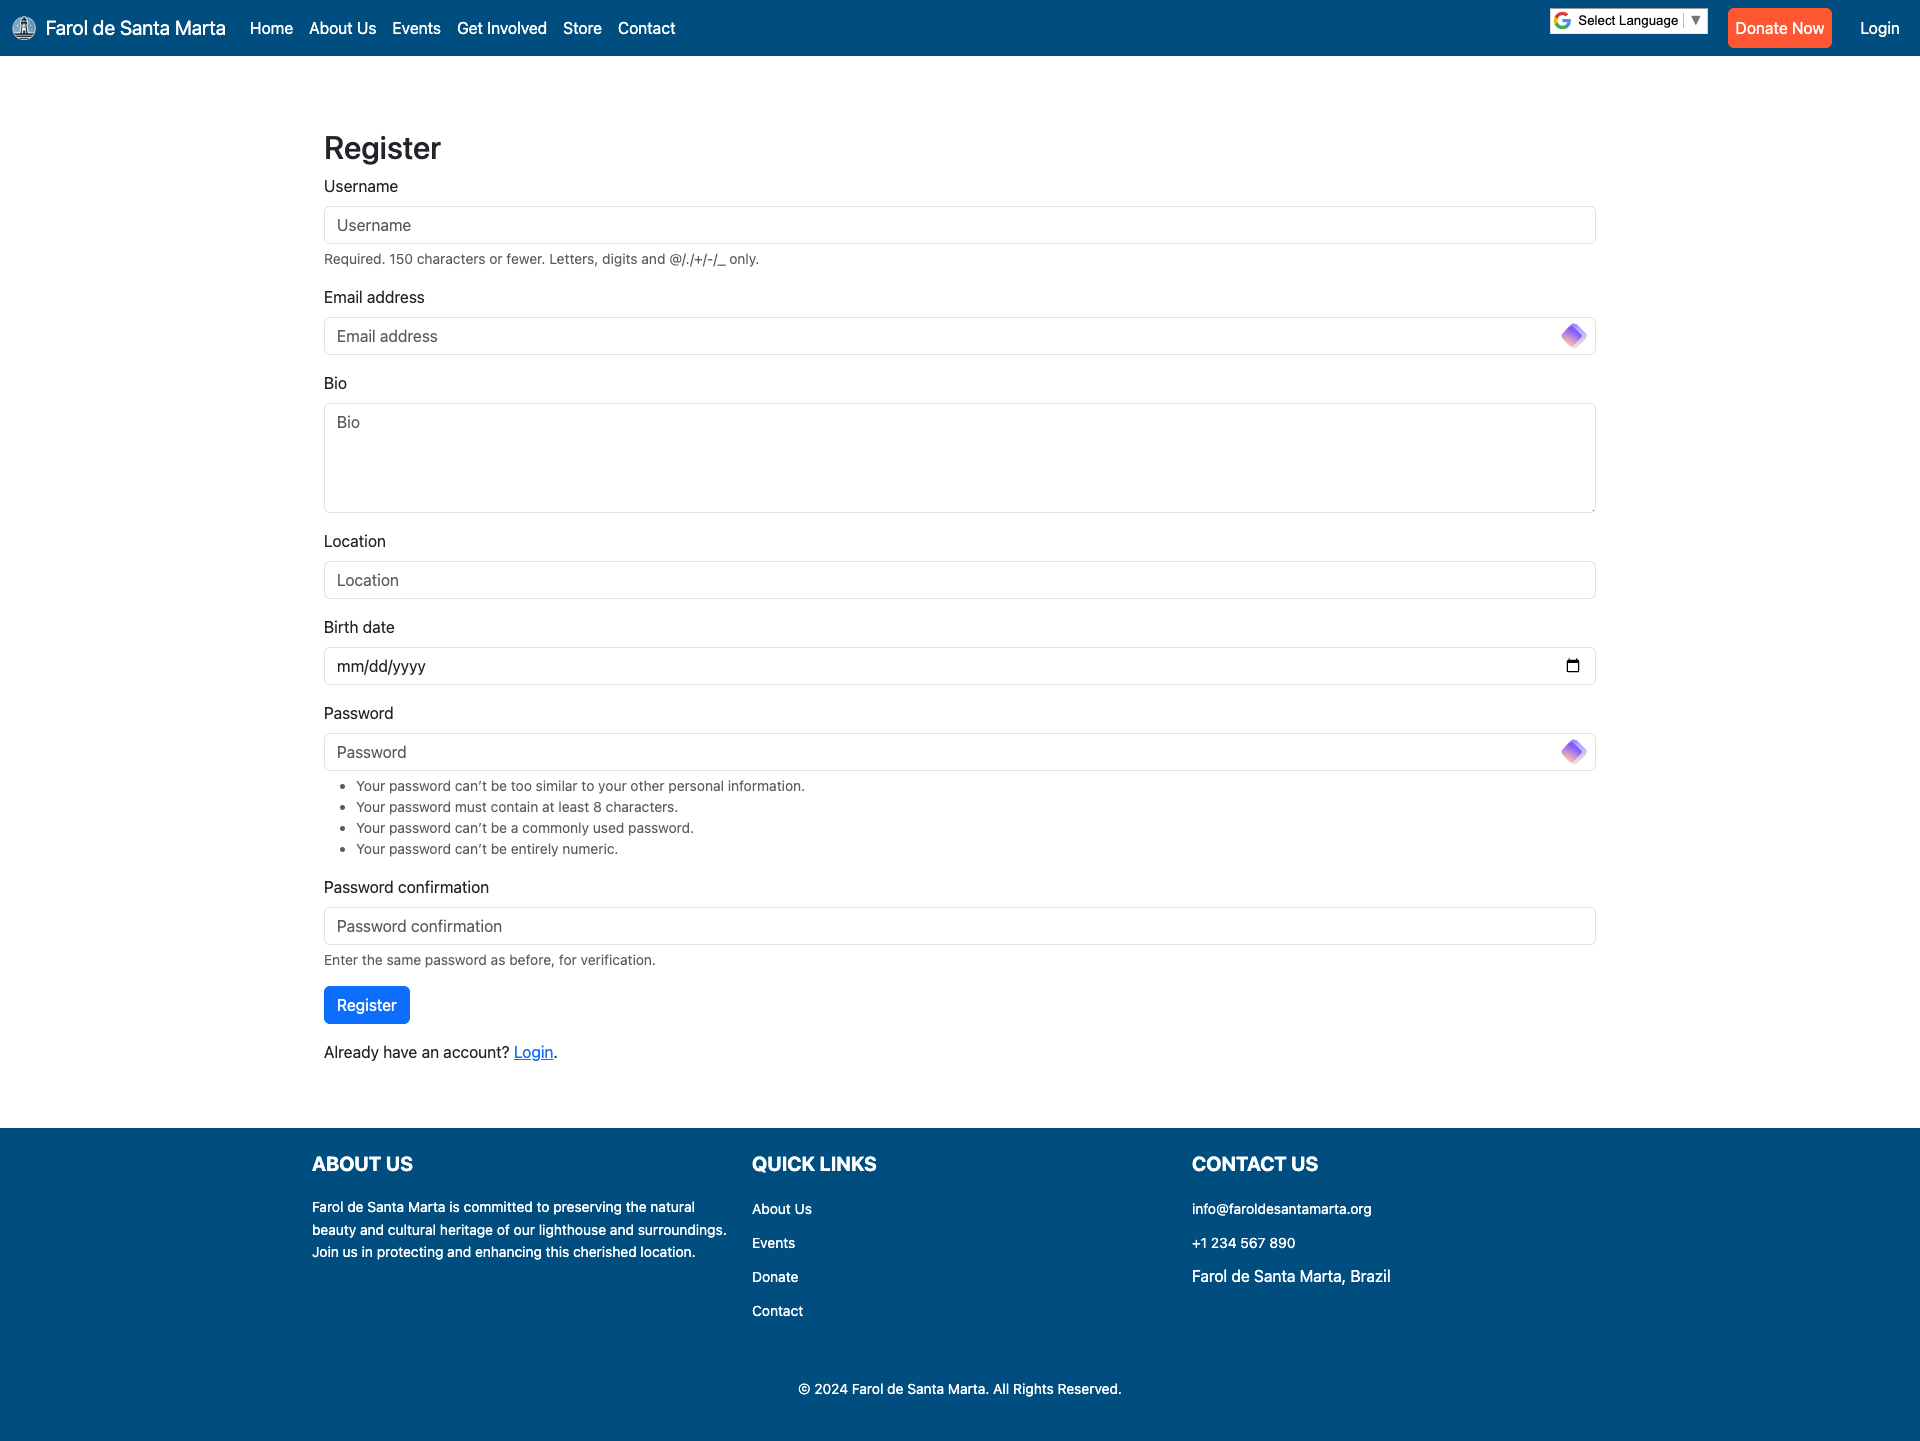
\includegraphics[width=\textwidth]{images/register-page.png}
    \caption{Example of the Register Page}
    \label{fig:register_page}
\end{figure}

\section{Technical Challenges}

During the development of the \textit{Farol de Santa Marta} website, several technical challenges were encountered, each requiring innovative solutions and persistent effort to overcome. This section discusses these challenges and the strategies employed to resolve them.

\subsection{Handling User Roles and Permissions}

Managing different user roles (e.g., students, teachers, and administrators) and their respective permissions presented a complex challenge, particularly in ensuring that each role had access only to the appropriate sections of the website.

This challenge was addressed by utilizing Django’s built-in user authentication and authorization system. Custom middleware was developed to enforce role-based access control, ensuring that users could only access pages and perform actions appropriate to their roles. Additionally, extensive testing was conducted to verify that the role-based permissions were correctly enforced across all features of the website.

\subsection{Database Design and Optimization}

Designing a robust database schema that could efficiently handle user data, course information, event details, and transaction records was a non-trivial task. The database needed to be optimized for performance while maintaining data integrity.

SQLite was selected as the database due to its simplicity and ease of integration with Django. The database schema was carefully designed to minimize redundancy and ensure efficient query performance. Indexing was implemented where necessary to speed up data retrieval, and Django’s ORM was used to manage database interactions securely and efficiently.

\section{GitHub Logs}

The GitHub logs provide a detailed record of all commits, showcasing the progress of the project from initial setup to final deployment. These logs are essential for understanding the development timeline and identifying significant milestones.

\begin{figure}[H]
    \centering
    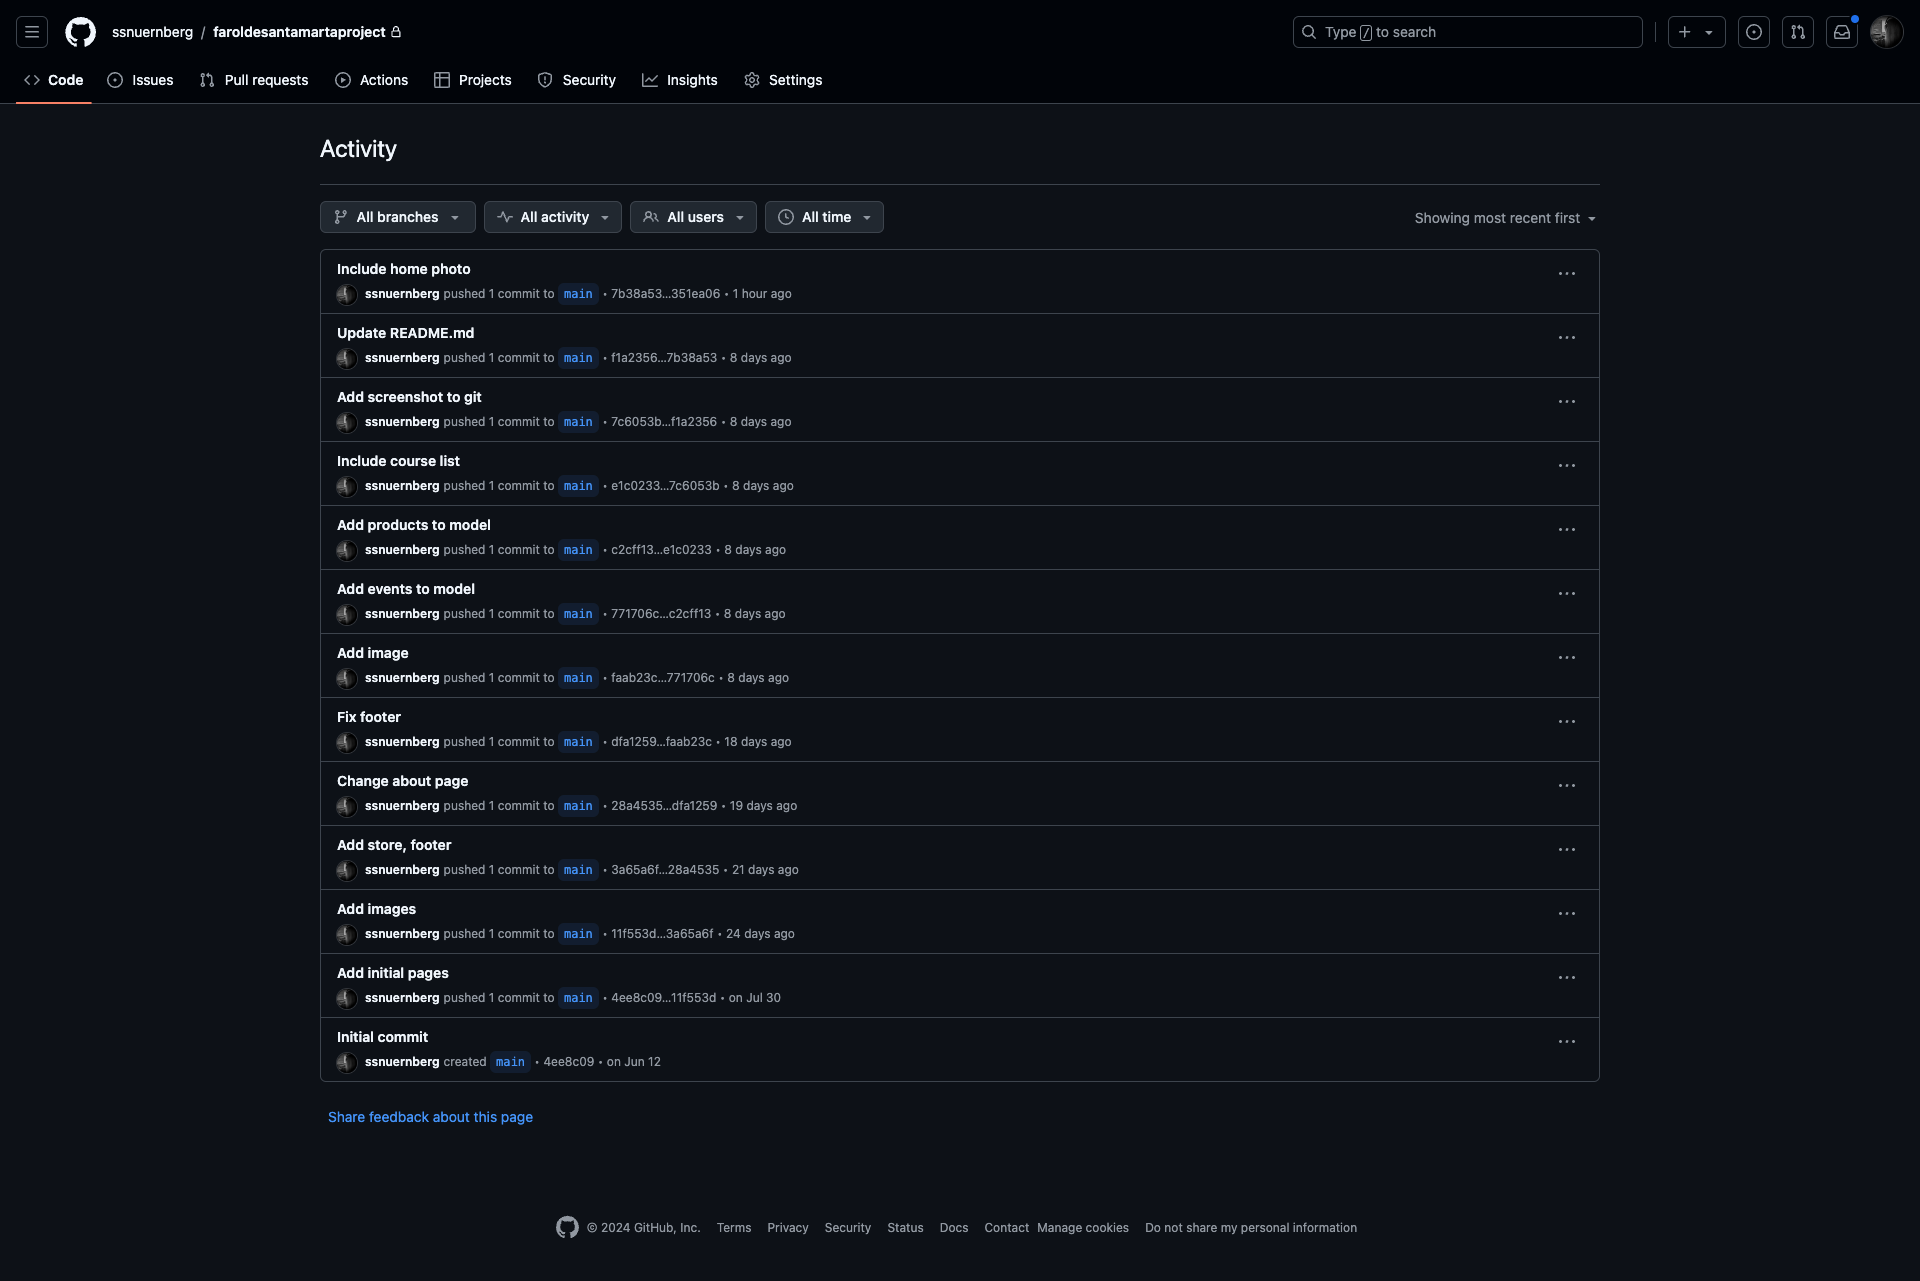
\includegraphics[width=\textwidth]{images/github-log.png}
    \caption{GitHub Logs of the \textit{Farol de Santa Marta} Project}
    \label{fig:github_logs}
\end{figure}

The logs illustrate the iterative nature of the development process. Key features such as user authentication, course management, and the donation system were developed incrementally, with regular commits ensuring that the project remained on track and aligned with the goals set out in the project plan.

The image in Figure \ref{fig:github_logs} provides a visual representation of the commit history, reflecting the steady progress and active development that characterized the \textit{Farol de Santa Marta} project.

The project will be public for access when published at \url{https://github.com/ssnuernberg/faroldesantamartaproject} and \url{http://www.faroldesantamarta.org}.



%%% Local Variables:
%%% mode: latex
%%% TeX-master: "../../main"
%%% End:
\chapter{Software testing}
\label{ch:testing}

% Choose your own headings.
\section{Testing Strategy}

To ensure the reliability, maintainability, and overall quality of the \textit{Farol de Santa Marta} website, a comprehensive testing strategy was implemented. The testing approach focused on validating the core functionalities of the application, ensuring that each component worked as intended and that the system as a whole performed reliably under various conditions.

\subsection{Testing Approach}

The testing strategy employed for this project included several layers of testing, each targeting different aspects of the application:

\subsubsection{Unit Testing}

Unit tests were developed to validate the functionality of individual components in isolation, particularly the models, views, and forms. These tests were designed to ensure that each function or method produced the expected output given a specific input. By testing each component independently, unit testing helped to identify and fix bugs early in the development process, reducing the likelihood of issues in the final product.

The \texttt{models.py}, \texttt{views.py}, and \texttt{urls.py} files located in the \texttt{tests/} subdirectory contain the implementation of these unit tests. The tests cover critical aspects such as:

\begin{itemize}
    \item Models: Ensuring data integrity and validation rules for user profiles, courses, events, feedback, and products.
    \item Views: Verifying that each view returns the correct HTTP response, renders the appropriate template, and interacts correctly with the models.
    \item Forms: Testing form validation logic, including required fields, data formats, and custom validation methods.
    \item User Flows: Simulating typical user actions such as registration, course enrollment, and making donations to ensure that these workflows operate smoothly from start to finish.
\end{itemize}

\subsubsection{Integration Testing}

Integration tests were conducted to evaluate the interaction between different components of the system. Unlike unit tests, which isolate individual components, integration tests assess how components work together to accomplish broader tasks. These tests focused on verifying that the system's components were properly integrated and that data flowed correctly between models, views, and templates.

For example, integration tests were used to verify that:

\begin{itemize}
    \item User registration and login processes correctly update the database and redirect users to the appropriate pages.
    \item Event creation and management features correctly interact with the database and are displayed accurately on the events page.
    \item The donation process integrates seamlessly with the payment gateway, and that transaction records are correctly stored.
\end{itemize}

\subsubsection{End-to-End Testing}

End-to-end (E2E) tests were employed to simulate real user interactions with the system from start to finish. These tests ensured that the entire application, from the frontend to the backend, worked together as expected in real-world scenarios. E2E testing was crucial for validating user workflows and ensuring that the application met its functional requirements.

Some of the key user flows tested through E2E testing included:

\begin{itemize}
    \item User registration and profile management.
    \item Browsing and enrolling in courses.
    \item Participating in events and providing feedback.
    \item Making purchases from the store and donating to conservation efforts.
\end{itemize}

\subsection{Automation and Continuous Integration}

To streamline the testing process and ensure consistent quality, tests were automated and integrated into the continuous integration (CI) pipeline. This approach allowed for automated testing whenever new code was pushed to the repository, ensuring that any issues were promptly identified and addressed before merging changes into the main codebase.


%%% Local Variables:
%%% mode: latex
%%% TeX-master: "../../main"
%%% End:

\chapter{Evaluation}
\label{ch:evaluation}

% Choose your own headings.
\section{User Testing}

\subsubsection{Usability Testing}

Usability testing was conducted to assess how easily and effectively users could navigate and interact with the website. A group of test users, representing the target audience of the website—including local community members, tourists, environmental activists, and students—were asked to perform specific tasks such as registering on the platform, enrolling in a course, participating in an event, and making a donation.

\textbf{Methodology:}

\begin{itemize}
    \item \textbf{Task Scenarios:} Participants were given predefined scenarios to complete, such as signing up for a beach clean-up event or purchasing an eco-friendly product from the store.
    \item \textbf{Observation:} User interactions were observed, and notes were taken on any difficulties encountered, areas of confusion, and overall user satisfaction.
    \item \textbf{Surveys and Feedback:} After completing the tasks, users were asked to fill out a survey rating their experience on various aspects such as ease of use, navigation, and visual design. Additional feedback was gathered through open-ended questions to identify areas for improvement.
\end{itemize}

\textbf{Findings:}

The usability testing revealed that the majority of users found the website intuitive and easy to navigate. Some minor issues were identified, such as the need for clearer labeling on certain buttons and the simplification of the donation process. These insights led to refinements in the user interface, ensuring that the website better aligned with user expectations and needs.

\subsection{Agile Methodology and Iterative Feedback}

The development of the \textit{Farol de Santa Marta} website was guided by Agile methodology, which emphasizes iterative development, continuous user feedback, and flexibility in responding to change. This approach allowed the developer to engage users throughout the process, ensuring that the website met their needs and expectations.

\textbf{User Testing and Feedback Loop:}

During one of the user testing sessions, participants highlighted the need for a more visually engaging homepage. Specifically, users suggested adding an image that represents the essence of Farol de Santa Marta, to better capture the attention of visitors and convey the website's mission.

\textbf{Outcome:}

The inclusion of the image improved the aesthetics of the homepage, ultimately enhancing their overall experience. This iterative process of testing and refinement, core to Agile practices, proved essential in developing a user-centered platform that effectively supports the goals of the \textit{Farol de Santa Marta} project.

\section{Critical Analysis}

In this section, the results of the \textit{Farol de Santa Marta} project are critically analyzed in relation to the project's goals. The discussion focuses on what worked well throughout the development and implementation phases, as well as identifying areas that could be improved in future iterations.

\subsection{Analysis of Results in Relation to Project Goals}

The primary goals of the \textit{Farol de Santa Marta} project were to create a user-friendly, secure, and scalable platform that supports environmental conservation efforts in the local community. These objectives were largely met, as evidenced by the successful deployment of the website and positive feedback from user testing.

\textbf{Goal 1: User Engagement and Accessibility}

One of the key objectives was to ensure that the website was accessible to a wide audience, including local residents, tourists, environmental activists, and students. The usability testing indicated that the website is intuitive and easy to navigate, with users able to complete key tasks such as event registration, course enrollment, and donations with minimal difficulty. The implementation of a responsive design also ensured that the site could be accessed on a variety of devices, further supporting the goal of broad accessibility.

\textbf{Goal 2: Support for Environmental Initiatives}

The project aimed to facilitate environmental conservation efforts through features such as event management, educational resources, and a donation system. The system’s ability to handle event creation and management and course enrollment indicates that these goals were effectively met. User feedback confirmed that the platform successfully supports the community's conservation efforts by providing essential tools and resources.

\subsection{What Worked Well}

Several aspects of the project were particularly successful:

\begin{itemize}
    \item \textbf{Agile Development Process:} The use of Agile methodology allowed for continuous feedback and iterative improvements. This approach ensured that the project remained aligned with user needs and could adapt to changing requirements.
    \item \textbf{Responsive Design:} The decision to implement a responsive design from the outset ensured that the website provided a consistent and accessible experience across different devices. This contributed significantly to user satisfaction.
\end{itemize}

\subsection{Areas for Improvement}

Despite the successes, there are several areas where the project could be improved:

\begin{itemize}
    \item \textbf{Integration of Local Nonprofits:} The integration with local nonprofits for the donation process is still in development. Future efforts should focus on establishing partnerships with these organizations to fully realize the donation system's potential and ensure compliance with local regulations.
    \item \textbf{Expanded Educational Content:} While the courses page provides valuable resources, the content could be expanded to cover a wider range of environmental topics, potentially involving more local experts and educators in content creation.
    \item \textbf{Better implementation of donation:} The integration of a donation system is still in development.    
\end{itemize}

%%% Local Variables:
%%% mode: latex
%%% TeX-master: "../../main"
%%% End:

\chapter{Conclusions and further work}
\label{ch:conclusions}

\section{Summary of Work}

The \textit{Farol de Santa Marta} project was undertaken with the primary objective of developing a user-friendly, secure, and scalable platform to support environmental conservation efforts in the Farol de Santa Marta community. The website aimed to engage local residents, tourists, environmental activists, and students in activities such as event participation, educational course enrollment, and donations to local conservation initiatives.

\section{Contributions}

The \textit{Farol de Santa Marta} project represents a significant contribution to the local community’s environmental conservation efforts. By providing an accessible and engaging platform, the project helps bridge the gap between community members and conservation activities. The originality of the project lies in its tailored approach to the specific needs of the Farol de Santa Marta community, combining best practices from global conservation platforms with a localized focus.

Moreover, the integration of educational resources and interactive features, such as course enrollment and event participation, not only raises awareness about environmental issues but also empowers users to take action. The platform’s design, which prioritizes user experience and accessibility, serves as a model for similar initiatives in other regions.

\section{Future Work}

While the \textit{Farol de Santa Marta} website successfully achieved its initial goals, there are several areas for potential improvement and extension:

\begin{itemize}
    \item \textbf{Expanded Educational Content}: Future iterations of the project could focus on expanding the range of educational materials available on the platform, including more courses on various environmental topics and involving more local experts in content creation.
    \item \textbf{Nonprofit Integration}: Strengthening partnerships with local nonprofits is crucial for fully realizing the donation system's potential. Future work should prioritize these collaborations to ensure that the platform remains compliant with local regulations and effectively channels donations to support conservation projects.
    \item \textbf{Better Implementation of Donation System}: The integration of a donation system is still in development. Future work should focus on fully implementing this feature, ensuring it is secure, user-friendly, and compliant with local regulations. This will involve collaborating with local nonprofits to streamline the process of receiving donations.
\end{itemize}


In conclusion, the \textit{Farol de Santa Marta} project has laid a strong foundation for ongoing and future environmental conservation efforts in the region. By addressing the areas for improvement and exploring potential extensions, the project can continue to evolve, making an even greater impact on the community and the environment.

%%% Local Variables:
%%% mode: latex
%%% TeX-master: "../../main"
%%% End:


% References

\printbibliography[heading=bibintoc]

% Appendices

%\appendix
%\chapter{Notational conventions}
\label{sec:notation}

\begin{center}
  \begin{tabular}{ll}
    \(S=\setof{\ldots}\) & the set \(S\)\\
    \(S \times S'\) & the Cartesian product of \(S\) and \(S'\)\\
    \(\rvert S \rvert\) & the cardinality of \(S\)\\
    \(\emptyset\) & the empty set\\
                         & \\
    \(\mathbb{R}\) & real numbers\\
    \(\mathbb{R^+}\) & positive real numbers\\
    \(\mathbb{R}^k\) & \nnk{-dimensional} real vector space\\
    \(\mathbb{Z}\) & integer numbers\\
    \(\mathbb{Z^+}\) & positive integer numbers\\
    \(\mathbb{N}\) & non-negative integer numbers\\
    \([x,y]\) & inclusive real-number interval between \(x\) and \(y\)\\
    \([x..y]\) & inclusive integer-number interval between \(x\) and \(y\)\\
                         & \\
    \(\vecb{v}=\tuple{\ldots}\) & the vector \(\vecb{v}\)\\
    \(\matb{M} = [m_{ij}]\) & the matrix \(\matb{M}\)\\
    \(\vecb{m}_i^j =\tuple{e_1, e_2, \ldots, e_j}\) & the ordered sequence of length \(j \in \mathbb{Z}^+\), indexed by \(i \le j\)\\
    \(\Vert\) & tuple concatenation: \(\tuple{0,1} \Vert \tuple{2,3} \to \tuple{0,1,2,3}\)\\
    \(\top\) & the symbol denoting undefined\\
  \end{tabular}
\end{center}


\end{document}
